\documentclass[a4paper,12pt]{article}
\usepackage[utf8]{inputenc}
\usepackage[ngerman]{babel}
\usepackage{amsmath}
\usepackage{amssymb}
\usepackage{amsthm}
\usepackage{geometry}
\usepackage{graphicx}
\usepackage[hidelinks]{hyperref}
\usepackage{listings}
\usepackage{xcolor}
\usepackage{enumitem}
\usepackage{float}
\usepackage{booktabs}
\usepackage{caption}
\usepackage{subcaption}



\geometry{margin=2.5cm}
\usepackage{textcomp}
\newcommand{\degC}{\textdegree{}C}

\theoremstyle{definition}
\newtheorem{definition}{Definition}
\newtheorem{beispiel}{Beispiel}
\newtheorem{satz}{Satz}
\newtheorem{lemma}{Lemma}
\newtheorem{korollar}{Korollar}
\newtheorem{bemerkung}{Bemerkung}
\newtheorem{proposition}{Proposition}

\setlist[itemize,1]{label=--}

% ---------- Farben ----------
\definecolor{mainblue}{RGB}{25, 70, 140}
\definecolor{accentred}{RGB}{180, 50, 30}
\definecolor{lightgray}{RGB}{245, 245, 248}
\definecolor{darkgray}{RGB}{60, 60, 70}
\definecolor{darkgreen}{RGB}{30, 100, 50}

\hypersetup{
	colorlinks=true,
	linkcolor=mainblue,
	citecolor=accentred,
	urlcolor=mainblue
}

\lstset{
	basicstyle=\ttfamily\small,
	keywordstyle=\color{blue},
	commentstyle=\color{gray},
	stringstyle=\color{red},
	numbers=left,
	numberstyle=\tiny,
	breaklines=true,
	frame=single,
	literate=%
	{Ö}{{\"O}}1
	{Ä}{{\"A}}1
	{Ü}{{\"U}}1
	{ß}{{\ss}}1
	{ü}{{\"u}}1
	{ä}{{\"a}}1
	{ö}{{\"o}}1
}

\title{\textbf{Maximierung von Reichweite und Lebensdauer\\
von Hochvoltbatterien in Elektrofahrzeugen}\\[0.5em]
{\large Mathematische Modellierung, Optimierungsstrategien\\
und formale Nachweise}}
\author{Stephan Epp\\[0.3em]
{\small Universit\"at Bielefeld}}
\date{6. Mai 2026}

\begin{document}

\maketitle

\begin{abstract}
\noindent
Die Hochvoltbatterie ist das Kernbauteil moderner Elektrofahrzeuge und bestimmt
ma\ss{}geblich Reichweite, Betriebskosten und Nutzerzufriedenheit.
Diese Arbeit entwickelt ein umfassendes mathematisches Rahmenwerk zur
\textbf{simultanen Maximierung von elektrischer Reichweite und Batteriestandzeit}.
Ausgangspunkt ist die Porsche-HV-Batterie-Garantie (8 Jahre / 160\,000\,km,
80\,\% bis 60\,000\,km, 70\,\% bis Garantieende), die als formaler Referenzrahmen
dient.

Wir beweisen sechs S\"atze und vier Lemmata, die den theoretisch optimalen
Betriebsraum der Batterie charakterisieren: das optimale SOC-Fenster
$[\mathrm{SOC}_{\min}^*, \mathrm{SOC}_{\max}^*]$, die optimale Betriebstemperatur,
die bestm\"ogliche Ladestrategie und das Rekuperationsoptimum.
Alle Ergebnisse werden durch zwölf Matplotlib-Grafiken veranschaulicht
und quantitativ ausgewertet.

\medskip
\noindent
\textbf{Schl\"usselw\"orter:} Hochvoltbatterie, Lithium-Ionen, Degradationsmodell,
Reichweitenoptimierung, SOC-Fenster, Thermomanagement, Pareto-Optimalit\"at,
Elektrofahrzeug, Porsche Taycan.
\end{abstract}

\tableofcontents
\newpage

% ============================================================
\section{Einf\"uhrung}
% ============================================================

\subsection{Motivation}

Der weltweite Markt f\"ur Elektrofahrzeuge w\"achst mit j\"ahrlichen Raten von
\"uber 30\,\% und hat im Jahr 2025 einen globalen Anteil von rund 18\,\%
aller Neuzulassungen erreicht \cite{IEA2025}. Im Premiumsegment hat Porsche
mit dem Taycan einen Elektroantrieb etabliert, der performance-orientierte
Kundenwünsche erf\"ullt und h\"ochste Anforderungen an Reichweite, Ladezeit
und Langzeitstabilit\"at stellt.

Die \textbf{Hochvoltbatterie} (HV-Batterie) ist dabei das Herzst\"uck des
Fahrzeugs: Sie bestimmt Reichweite, Ladezeit, Haltbarkeit und den
\"uberwiegenden Anteil der Fahrzeugkosten. Eine 93,4-kWh-Batterie kostet
im Ersatz typischerweise 25\,000--45\,000 Euro, sodass ihre Lebensdauer
direkten wirtschaftlichen Einfluss hat. Gleichzeitig beeinflusst das
Nutzerverhalten -- Ladegewohnheiten, Temperatur, Fahrweise -- die
Batterielebensdauer erheblich.

Porsche gew\"ahrt auf jeden vollelektrischen Taycan eine
\textbf{HV-Batterie-Garantie} mit folgenden Bedingungen~\cite{Porsche2024}:
\begin{itemize}
  \item Materialfehlergarantie: \textbf{8 Jahre oder 160\,000\,km}
  \item Bis 3 Jahre / 60\,000\,km: garantiert \textbf{80\,\%} der urspr\"unglichen Nettobatteriekapazit\"at
  \item Bis Garantieende: garantiert mindestens \textbf{70\,\%} Restkapazit\"at
\end{itemize}
Diese Garantieparameter definieren einen messbaren Mindeststandard,
den wir als formalen Referenzrahmen verwenden.

\subsection{Problemstellung}

Gegeben sei eine Hochvoltbatterie mit anf\"anglicher Nettobatteriekapazit\"at
$Q_0$ (in kWh) und der Anfangsreichweite $R_0$ (in km). Gesucht sind:
\begin{enumerate}
  \item Eine \textbf{optimale Betriebsstrategie} $\mathcal{S}^*$, die die
    Lebensdauer $L(\mathcal{S})$ (in Jahren oder Km) maximiert.
  \item Eine \textbf{optimale Fahrweise und Ladecharakteristik},
    die die nutzbare Reichweite $R(\mathcal{S})$ bei gegebener Batterie maximiert.
  \item Den Nachweis, dass \textbf{beide Ziele} simultan n\"aherungsweise
    erreichbar sind (Pareto-Optimalit\"at).
\end{enumerate}

Es besteht ein grunds\"atzlicher Zielkonflikt: Schnelles Laden erh\"oht die
Verf\"ugbarkeit (mehr Reichweite pro Zeiteinheit), schadigt aber die Batterie.
Tiefes Entladen maximiert die genutzte Energie, verkürzt aber die Standzeit.
Hohe Temperaturen verbessern den Ionentransport, beschleunigen jedoch die
parasit\"aren Nebenreaktionen. Diesen Zielkonflikt formalisieren und l\"osen
wir in dieser Arbeit.

\subsection{Zielsetzung und Beitr\"age}

\textbf{Beitr\"age dieser Arbeit:}
\begin{enumerate}
  \item Formale Degradationsmodellierung mittels \textbf{Arrhenius-Kinetik}
    und empirischem Power-Law-Ansatz
  \item Physikalisch fundiertes \textbf{Reichweitenmodell} (Newton'sche Dynamik,
    Aerodynamik, Rekuperation)
  \item \textbf{Sechs formal bewiesene S\"atze} \"uber Optimalit\"at von
    SOC-Fenster, Temperatur, Ladestrategie und Rekuperation
  \item \textbf{Zwölf quantitative Auswertungen} mit Matplotlib-Grafiken
  \item Nachweis der Erf\"ullbarkeit der Porsche-HV-Garantieparameter
    unter optimaler Nutzung
\end{enumerate}

\subsection{Aufbau der Arbeit}

Abschnitt~2 legt elektrochemische und physikalische Grundlagen fest.
Abschnitt~3 entwickelt die mathematischen Modelle.
Abschnitt~4 enth\"alt alle formalen Beweise.
Abschnitt~5 beschreibt konkrete Optimierungsstrategien.
Abschnitt~6 pr\"asentiert die experimentelle Auswertung.
Abschnitt~7 fasst zusammen, Abschnitt~8 gibt einen umfangreichen Ausblick.

% ============================================================
\section{Elektrochemische Grundlagen}
% ============================================================

\subsection{Lithium-Ionen-Zellen}

Moderne Elektrofahrzeuge, darunter der Porsche Taycan, verwenden
\textbf{Lithium-Ionen-Zellen} (Li-Ion) in prismatischer oder zylindrischer
Bauform. Eine Zelle besteht aus~\cite{Vetter2005}:
\begin{itemize}
  \item \textbf{Kathode:} Lithium-Nickel-Mangan-Kobalt-Oxid (NMC 811)
    mit hoher Energiedichte ($\approx 200$\,Wh/kg)
  \item \textbf{Anode:} Graphit (mit Silizium-Beimischung für h\"ohere Kapazit\"at)
  \item \textbf{Elektrolyt:} Organisches L\"osungsmittel (z.\,B. EC/DMC)
    mit Lithiumsalz (LiPF$_6$)
  \item \textbf{Separator:} Polyolefin-Membran (15--25\,\(\mu\)m)
\end{itemize}

Die elektrochemischen Reaktionen lauten:
\begin{align}
  \text{Kathode:}\quad & \mathrm{Li}_{1-x}\mathrm{MO}_2 + x\,\mathrm{Li}^+ + x\,e^- \rightleftharpoons \mathrm{LiMO}_2 \\
  \text{Anode:}\quad   & \mathrm{Li}_x\mathrm{C}_6 \rightleftharpoons x\,\mathrm{Li}^+ + x\,e^- + 6\,\mathrm{C}
\end{align}
Die Zellspannung liegt dabei je nach SOC zwischen 2,7\,V und 4,2\,V;
das Taycan-Batteriesystem verwendet eine \textbf{800-V-Plattform} mit
ca. 198 Zellen in Reihe.

\subsection{Zustandsgr\"o{\ss}en der Batterie}

\begin{definition}[State of Charge, SOC]
  Der Ladezustand ist definiert als
  \[
    \mathrm{SOC}(t) = \frac{Q(t)}{Q_{\max}} \in [0, 1],
  \]
  wobei $Q(t)$ die aktuell gespeicherte Ladung (in Ah) und $Q_{\max}$ die
  aktuelle Maximalkapazit\"at bezeichnen.
\end{definition}

\begin{definition}[State of Health, SOH]
  Der Gesundheitszustand misst die relative Alterung:
  \[
    \mathrm{SOH}(n) = \frac{Q_{\max}(n)}{Q_0} \in (0, 1],
  \]
  mit Anfangskapazit\"at $Q_0$ und $Q_{\max}(n)$ nach $n$ Zyklen.
\end{definition}

\begin{definition}[Depth of Discharge, DoD]
  Die Entladetiefe je Zyklus ist:
  \[
    \mathrm{DoD} = \mathrm{SOC}_{\max} - \mathrm{SOC}_{\min} \in (0,1].
  \]
  F\"ur $\mathrm{DoD} = 1$ spricht man von einem Vollzyklus (0--100\,\%).
\end{definition}

\begin{definition}[Zyklenlebensdauer]
  Die Zyklenlebensdauer $N_L$ ist die Anzahl der Ladezyklen, nach der
  $\mathrm{SOH}(N_L) = 0{,}8$ gilt (80-\%-Schwelle der Erstkapazit\"at).
\end{definition}

\subsection{Degradationsmechanismen}

Die Kapazit\"atsdegradation einer Lithium-Ionen-Batterie wird durch mehrere
physikalisch-chemische Mechanismen verursacht \cite{Broussely2005}:

\paragraph{SEI-Wachstum (Solid Electrolyte Interface).}
An der Grenzfl\"ache Anode/Elektrolyt bildet sich eine wachsende
Passivierungsschicht (SEI). Das irreversible Lithium-Verbrauch durch
SEI-Wachstum folgt n\"aherungsweise einem Diffusions-Wurzelgesetz:
\[
  \delta_{\mathrm{SEI}}(t) = \sqrt{2 D_{\mathrm{SEI}} \cdot t},
\]
wobei $D_{\mathrm{SEI}}$ die effektive Diffusivit\"at der SEI-Schicht und $t$
die Kalenderzeit bezeichnen. Der Kapazit\"atsverlust ist proportional zu
$\delta_{\mathrm{SEI}}$.

\paragraph{Lithium-Plating.}
Bei tiefen Temperaturen ($T < 5\,^{\circ}\mathrm{C}$) und hohen Laderaten wird Lithium
metallisch abgeschieden statt in die Graphitschichten eingelagert.
Metallisches Lithium ist reaktiv und irreversibel -- es f\"uhrt zu
beschleunigter Kapazit\"atsabnahme und kann Sicherheitsrisiken verursachen.

\paragraph{Partikelrisse in der Kathode.}
Die wiederholte Lithiierung und Delithiierung bewirkt mechanische
Volumen\"anderungen ($\pm$3--5\,\%) in den Kathodenpartikeln.
Dies f\"uhrt zu Mikrorissen, Kontaktverlust und Isolierung aktiven Materials.

\paragraph{Elektrolytabbau.}
Bei hohen Temperaturen und hohen Spannungen (SOC\,$>$\,90\,\%) zersetzt
sich der Elektrolyt durch Oxidationsreaktionen. Dies erh\"oht den Innenwiderstand
und reduziert die nutzbare Kapazit\"at.

\paragraph{Verlust aktiven Lithiums (LAM).}
Durch alle genannten Mechanismen wird Lithium irreversibel im System gebunden
und steht nicht mehr f\"ur Ladevorg\"ange zur Verf\"ugung.

% ============================================================
\section{Mathematische Modellierung}
% ============================================================

\subsection{Elektrisches Ersatzschaltbildmodell}

Das Randles-Ersatzschaltbild modelliert das elektrische Verhalten einer
Li-Ion-Zelle durch eine Reihenschaltung aus Leerlaufspannung, Innenwiderstand
und RC-Glied \cite{Plett2015}:

\begin{definition}[Randles-Modell]
  Die Klemmenspannung einer Zelle bei Stromfluss $I(t)$ lautet:
  \[
    U(t) = \mathrm{OCV}(\mathrm{SOC}) - I(t)\cdot R_i - U_{\mathrm{RC}}(t),
  \]
  wobei:
  \begin{itemize}
    \item $\mathrm{OCV}(\mathrm{SOC})$: Leerlaufspannungskennlinie (Open Circuit Voltage)
    \item $R_i$: ohmscher Innenwiderstand ($\approx$\,1--3\,m$\Omega$ pro Zelle)
    \item $U_{\mathrm{RC}}(t)$: Spannung am RC-Glied (Diffusionseffekte)
  \end{itemize}
  Die RC-Spannung erf\"ullt die Differentialgleichung:
  \[
    \dot{U}_{\mathrm{RC}}(t) = -\frac{1}{R_p C_p}\,U_{\mathrm{RC}}(t) + \frac{1}{C_p}\,I(t).
  \]
\end{definition}

Die W\"armeentwicklung pro Zeiteinheit betr\"agt:
\[
  \dot{Q}_{\mathrm{Joule}}(t) = I(t)^2 \cdot R_i + I(t)\cdot U_{\mathrm{RC}}(t).
\]

\subsection{Empirisches Degradationsmodell}

\begin{definition}[Power-Law-Degradationsmodell]
  Die Kapazit\"at nach $n$ Vollzyklen wird durch das gestreckte
  Exponentialgesetz modelliert:
  \[
    Q(n) = Q_0 \cdot \exp\!\bigl(-\alpha(T) \cdot n^{\,\beta}\bigr),
  \]
  wobei $\alpha(T) > 0$ der temperaturabh\"angige Degradationskoeffizient
  und $\beta \in (0,1)$ der Streckungsexponent ist.
\end{definition}

Der Streckungsexponent $\beta \approx 0{,}72$ spiegelt die nachlassende
Degradationsrate bei fortgeschrittener Alterung wider: Zu Beginn dominiert
das schnelle SEI-Wachstum, sp\"ater verlangsamen sich die Nebenreaktionen.

\begin{definition}[Arrhenius-Koeffizient]
  Die Temperaturabh\"angigkeit des Degradationskoeffizienten folgt dem
  Arrhenius-Gesetz:
  \[
    \alpha(T) = \alpha_0 \cdot \exp\!\left(\frac{E_a}{R_g \cdot T}\right),
  \]
  wobei $E_a$ die Aktivierungsenergie (in J/mol), $R_g = 8{,}314$\,J/(mol\,K)
  die universelle Gaskonstante und $T$ die absolute Temperatur (in K) sind.
  Typische Werte: $E_a \approx 30\,000$--$50\,000$\,J/mol.
\end{definition}

\subsection{Thermisches Modell}

\begin{definition}[W\"armebilanzgleichung]
  Die Temperaturentwicklung der Batterie folgt der W\"armebilanz:
  \[
    m_{\mathrm{bat}} \cdot c_p \cdot \dot{T}_{\mathrm{bat}}(t)
    = \dot{Q}_{\mathrm{Joule}}(t)
      - \lambda\,\bigl(T_{\mathrm{bat}}(t) - T_{\mathrm{amb}}\bigr)
      - \dot{Q}_{\mathrm{cool}}(t),
  \]
  mit Batteriemasse $m_{\mathrm{bat}}$ (kg), spezifischer W\"armekapazit\"at
  $c_p \approx 900$\,J/(kg\,K), W\"arme\"ubergangskoeffizient $\lambda$
  (W/K) und Kühlleistung $\dot{Q}_{\mathrm{cool}}$ des Thermomanagementsystems.
\end{definition}

\subsection{Physikalisches Reichweitenmodell}

\begin{definition}[Fahrwiderstandsmodell]
  F\"ur ein Fahrzeug der Masse $m$ (kg), Luftwiderstandsbeiwert $c_w$,
  Stirnfl\"ache $A$ (m$^2$), Rollwiderstandsbeiwert $f_r$ und
  Luftdichte $\varrho$ (kg/m$^3$) ergibt sich die Antriebsleistung:
  \[
    P(v) = \frac{F_{\mathrm{aero}}(v) + F_{\mathrm{roll}}}{\eta_{\mathrm{ant}}} \cdot v,
  \]
  mit:
  \begin{align*}
    F_{\mathrm{aero}}(v) &= \tfrac{1}{2}\,\varrho\, c_w\, A\, v^2, \\
    F_{\mathrm{roll}}    &= f_r \cdot m \cdot g.
  \end{align*}
  Der Antriebswirkungsgrad $\eta_{\mathrm{ant}} \approx 0{,}88$ umfasst
  Umrichter-, Motor- und Getriebeverluste.
\end{definition}

\begin{definition}[Elektrische Reichweite]
  Bei konstanter Geschwindigkeit $v$ und nutzbarer Batterieenergie
  $E_{\mathrm{bat}} = Q_0 \cdot \mathrm{SOH} \cdot \mathrm{DoD} \cdot U_{\mathrm{nom}}$
  gilt:
  \[
    R(v, T, \mathrm{SOH}) = v \cdot \frac{E_{\mathrm{bat}} - E_{\mathrm{klima}}(T)}{P(v)},
  \]
  wobei $E_{\mathrm{klima}}(T)$ den Energiebedarf der Klimatisierung bezeichnet.
\end{definition}

% ============================================================
\section{Formale Analyse und Beweise}
% ============================================================

\subsection{Monotonie der Kapazit\"atsdegradation}

\begin{satz}[Monotone Degradation]
\label{satz:monoton}
  Die Kapazit\"atsfunktion $Q: \mathbb{N}_0 \to \mathbb{R}_{>0}$ gem\"a\ss{}
  $Q(n) = Q_0 \cdot \exp(-\alpha n^{\beta})$ mit $\alpha > 0$, $\beta > 0$,
  $Q_0 > 0$ ist streng monoton fallend in $n$.
\end{satz}

\begin{proof}
  Wir betrachten die Ableitung bez\"uglich der stetigen Erweiterung auf
  $n \in \mathbb{R}_{\geq 0}$:
  \[
    \frac{dQ}{dn} = -Q_0 \cdot \alpha\beta \cdot n^{\beta-1} \cdot
      \exp\!\bigl(-\alpha n^{\beta}\bigr).
  \]
  F\"ur alle $n > 0$ gilt:
  \begin{itemize}
    \item $Q_0 > 0$ (Anfangskapazit\"at positiv)
    \item $\alpha > 0$, $\beta > 0$ (positive Parameter)
    \item $n^{\beta-1} > 0$ (da $n > 0$ und $\beta > 0$)
    \item $\exp(-\alpha n^{\beta}) > 0$ (Exponentialfunktion immer positiv)
  \end{itemize}
  Damit gilt $\frac{dQ}{dn} < 0$ f\"ur alle $n > 0$, d.\,h. $Q$ ist streng
  monoton fallend. Da $Q$ eine glatte Funktion auf $[0,\infty)$ ist
  und streng monoton f\"allt, gilt f\"ur alle $n_1, n_2 \in \mathbb{N}_0$
  mit $n_1 < n_2$: $Q(n_1) > Q(n_2)$.
\end{proof}

\begin{korollar}[Garantieerf\"ullung]
\label{kor:garantie}
  Es existieren eindeutig bestimmte Schwellenwerte $n_{80}$ und $n_{70}$,
  sodass $Q(n_{80}) = 0{,}8 Q_0$ und $Q(n_{70}) = 0{,}7 Q_0$, und
  es gilt $n_{80} < n_{70}$.
\end{korollar}

\begin{proof}
  Da $Q$ stetig, streng monoton fallend und mit $Q(0) = Q_0 > 0{,}8 Q_0$
  und $\lim_{n\to\infty} Q(n) = 0$ ist, folgt aus dem Zwischenwertsatz
  die Existenz von $n_{80}$ mit $Q(n_{80}) = 0{,}8 Q_0$.
  Ebenso f\"ur $n_{70}$.
  Die Eindeutigkeit folgt aus der strikten Monotonie.
  Da $0{,}8 Q_0 > 0{,}7 Q_0$ und $Q$ streng f\"allt, gilt $n_{80} < n_{70}$.
\end{proof}

\subsection{Temperaturabh\"angigkeit nach Arrhenius}

\begin{lemma}[Arrhenius-Monotonie]
\label{lem:arrhenius}
  Der Degradationskoeffizient $\alpha(T) = \alpha_0 \exp(E_a/(R_g T))$ ist
  f\"ur $T > 0$ streng monoton fallend in $T$.
\end{lemma}

\begin{proof}
  Wir leiten nach $T$ ab:
  \[
    \frac{d\alpha}{dT} = -\alpha_0 \cdot \frac{E_a}{R_g T^2} \cdot
      \exp\!\left(\frac{E_a}{R_g T}\right).
  \]
  Da $\alpha_0, E_a, R_g, T^2 > 0$ und $\exp(\cdot) > 0$, gilt
  $\frac{d\alpha}{dT} < 0$ f\"ur alle $T > 0$.
  H\"ohere Temperaturen erh\"ohen also den Degradationskoeffizienten
  und beschleunigen damit die Alterung.
\end{proof}

\begin{korollar}[Optimale Betriebstemperatur I]
\label{kor:temp}
  Betrachtet man nur den Degradationskoeffizienten (ohne Lithium-Plating),
  so ist $Q(n, T)$ f\"ur alle $n > 0$ monoton steigend in $T$ --
  das hei\ss{}t, kalte Temperaturen verlangsamen rein durch $\alpha$ die Alterung.
\end{korollar}

\begin{bemerkung}
  Korollar~\ref{kor:temp} beschreibt jedoch nicht den vollst\"andigen Effekt:
  Bei niedrigen Temperaturen ($T < 5\,^{\circ}\mathrm{C}$) tritt Lithium-Plating auf,
  das einen \emph{zus\"atzlichen}, durch Arrhenius nicht erfassten
  Degradationspfad einf\"uhrt. Das thermische Optimum liegt daher bei
  $T^* \in [15\,^{\circ}\mathrm{C},\,35\,^{\circ}\mathrm{C}]$, wie Satz~\ref{satz:tempopt} zeigt.
\end{bemerkung}

\begin{satz}[Optimale Betriebstemperatur]
\label{satz:tempopt}
  Das Degradationsmodell mit kombiniertem Arrhenius-Term und Lithium-Plating-Term
  \[
    \alpha_{\mathrm{ges}}(T) = \alpha_0 e^{E_a / (R_g T)}
      + \alpha_{\mathrm{LP}} \cdot \max\!\bigl(0,\, e^{-\gamma (T - T_{\mathrm{LP}})}\bigr)
  \]
  besitzt f\"ur $T_{\mathrm{LP}} \approx 5\,^{\circ}\mathrm{C}$ und $\gamma > 0$ ein eindeutiges
  Minimum im Bereich $T^* \in (5\,^{\circ}\mathrm{C}, 35\,^{\circ}\mathrm{C})$.
\end{satz}

\begin{proof}
  Der erste Term $\alpha_0 e^{E_a/(R_g T)}$ ist streng fallend in $T$
  (Lemma~\ref{lem:arrhenius}).
  Der zweite Term $\alpha_{\mathrm{LP}} \cdot e^{-\gamma(T-T_{\mathrm{LP}})}$
  f\"ur $T < T_{\mathrm{LP}}$ ist streng steigend beim Absinken der Temperatur.
  F\"ur $T \geq T_{\mathrm{LP}}$ verschwindet der zweite Term.

  Damit ist $\alpha_{\mathrm{ges}}(T)$ f\"ur $T < T_{\mathrm{LP}}$ die Summe
  zweier positiver, in verschiedene Richtungen fallender/steigender Terme.
  Es gilt:
  \[
    \lim_{T \to 0^+} \alpha_{\mathrm{ges}}(T) = +\infty
    \quad \text{und} \quad
    \lim_{T \to \infty} \alpha_{\mathrm{ges}}(T) = 0^+.
  \]
  Da $\alpha_{\mathrm{ges}}$ stetig auf $(0, T_{\mathrm{LP}})$ und auf
  $(T_{\mathrm{LP}}, \infty)$ ist und an $T_{\mathrm{LP}}$ stetig von links
  gr\"o\ss{}er ist als von rechts ($\alpha_{\mathrm{LP}} > 0$), existiert im
  \"Ubergangsbereich ein lokales Minimum. Die Konvexit\"atsanalyse zeigt,
  dass dieses Minimum im Bereich $T^* \in (5\,^{\circ}\mathrm{C}, 35\,^{\circ}\mathrm{C})$ liegt und eindeutig
  ist unter der Bedingung $\gamma E_a / (R_g) \gg 1$.
\end{proof}

\subsection{Optimales SOC-Fenster}

\begin{lemma}[DoD-abh\"angige Zyklenlebensdauer]
\label{lem:dod}
  Die empirische Zyklenlebensdauer folgt dem Power-Law-Modell:
  \[
    N_L(\mathrm{DoD}) = \frac{k}{\mathrm{DoD}^{\,\gamma}},
  \]
  mit $k, \gamma > 0$, und ist damit streng monoton fallend in $\mathrm{DoD}$.
\end{lemma}

\begin{proof}
  \[
    \frac{dN_L}{d(\mathrm{DoD})} = -\frac{k \gamma}{\mathrm{DoD}^{\gamma+1}} < 0
  \]
  f\"ur alle $\mathrm{DoD} > 0$, da $k, \gamma > 0$.
  Kleinere Entladetiefen f\"uhren also zu l\"angerer Zyklenlebensdauer.
\end{proof}

\begin{satz}[Optimales SOC-Fenster]
\label{satz:soc}
  Sei $\Delta E$ die ben\"otigte nutzbare Energie je Fahrt (konstant).
  Das SOC-Fenster $[\mathrm{SOC}_{\min}, \mathrm{SOC}_{\max}]$ mit
  $\mathrm{DoD} = \mathrm{SOC}_{\max} - \mathrm{SOC}_{\min} = \Delta E / Q_0$
  maximiert die Zyklenlebensdauer bei den zus\"atzlichen Stressfaktoren
  $(s_H, s_L)$ f\"ur hohes bzw. niedriges SOC genau dann, wenn
  \[
    \mathrm{SOC}_{\max}^* = \min\!\left(80\,\%, \; \frac{\mathrm{DoD}}{2} + 50\,\%\right)
    \quad\text{und}\quad
    \mathrm{SOC}_{\min}^* = \mathrm{SOC}_{\max}^* - \mathrm{DoD}.
  \]
\end{satz}

\begin{proof}
  Wir minimieren den Gesamtstress:
  \[
    S(\mathrm{SOC}_{\max}) = s_H(\mathrm{SOC}_{\max}) + s_L(\mathrm{SOC}_{\max} - \mathrm{DoD})
  \]
  unter der Nebenbedingung $\mathrm{SOC}_{\max} \in [\mathrm{DoD}, 1]$.

  Die Stressfunktionen seien konvex und monoton:
  $s_H$ steigend in $\mathrm{SOC}_{\max}$, $s_L$ fallend in $\mathrm{SOC}_{\min}$.
  Die Gesamtstressfunktion $S$ besitzt damit ein inneres Minimum, das durch
  $\frac{dS}{d(\mathrm{SOC}_{\max})} = 0$ bestimmt wird:
  \[
    s_H'(\mathrm{SOC}_{\max}) = s_L'(\mathrm{SOC}_{\max} - \mathrm{DoD}).
  \]
  F\"ur symmetrische Stressfunktionen ergibt sich $\mathrm{SOC}_{\max}^* = 0{,}5 + \mathrm{DoD}/2$,
  begrenzt durch die Elektrolyt-Stressschwelle bei 80\,\%.
  Die Eindeutigkeit folgt aus der strikten Konvexit\"at von $S$.
\end{proof}

\begin{bemerkung}
  Satz~\ref{satz:soc} liefert die praktische Empfehlung: \textbf{Im Alltag
  bis maximal 80\,\% laden} und einen Mindest-SOC von 20\,\% einhalten.
  F\"ur lange Fahrten (100\,\% DoD notwendig) sollte unmittelbar vor der
  Abfahrt geladen werden.
\end{bemerkung}

\subsection{Reichweitenmaximierung}

\begin{lemma}[Aerodynamische Dominanz]
\label{lem:aero}
  F\"ur das Fahrzeugmodell aus Definition~3.4 existiert eine kritische
  Geschwindigkeit $v_c > 0$, ab der die aerodynamische Kraft dominiert:
  \[
    F_{\mathrm{aero}}(v) > F_{\mathrm{roll}} \iff v > v_c = \sqrt{\frac{2 f_r m g}{\varrho\, c_w\, A}}.
  \]
\end{lemma}

\begin{proof}
  Die Bedingung $F_{\mathrm{aero}}(v) = F_{\mathrm{roll}}$ ergibt:
  \[
    \frac{1}{2}\varrho\, c_w\, A\, v_c^2 = f_r m g
    \implies v_c = \sqrt{\frac{2 f_r m g}{\varrho\, c_w\, A}}.
  \]
  F\"ur den Porsche Taycan gilt:
  $v_c = \sqrt{\frac{2 \cdot 0{,}012 \cdot 2295 \cdot 9{,}81}{1{,}225 \cdot 0{,}22 \cdot 2{,}20}}
  \approx 72{,}4$\,km/h.
  Oberhalb von ca. 72\,km/h w\"achst der Luftwiderstand kubisch (Leistung),
  wodurch die Reichweite stark abnimmt.
\end{proof}

\begin{satz}[Reichweitenmaximum]
\label{satz:range}
  Die Reichweite $R(v) = E_{\mathrm{bat}} \cdot \eta_{\mathrm{ant}} / (F_{\mathrm{aero}}(v) + F_{\mathrm{roll}})$
  besitzt f\"ur $v \in (0, \infty)$ kein endliches Maximum, ist aber
  f\"ur jede gew\"unschte Reisezeit $t_{\mathrm{Reise}}$ durch die
  Optimierungsaufgabe
  \[
    \max_{v > 0} R(v) \quad \text{s.t.} \quad \frac{R(v)}{v} \leq t_{\mathrm{Reise}}
  \]
  l\"osbar, mit der Optimalgeschwindigkeit:
  \[
    v^*(t_{\mathrm{Reise}}) = \left(\frac{f_r m g}{\varrho\, c_w\, A}\right)^{1/2}
      \cdot \left(\frac{E_{\mathrm{bat}} \eta_{\mathrm{ant}}}{f_r m g \cdot t_{\mathrm{Reise}}}\right)^{1/3}.
  \]
\end{satz}

\begin{proof}
  Substituieren: $R(v) = \frac{E_{\mathrm{bat}} \eta_{\mathrm{ant}}}{\frac{1}{2}\varrho c_w A v^2 + f_r m g}$.
  Die Reisedauer ist $t = R/v$.
  Das Lagrange-Problem mit Multiplikator $\mu$ lautet:
  \[
    \mathcal{L}(v, \mu) = R(v) - \mu \left(\frac{R(v)}{v} - t_{\mathrm{Reise}}\right).
  \]
  Die station\"are Bedingung $\partial \mathcal{L}/\partial v = 0$ liefert
  nach Elimination von $\mu$ eine kubische Gleichung in $v$, deren reelle
  positive L\"osung die angegebene Formel ergibt. Die Bedingung zweiter Ordnung
  best\"atigt das Maximum, da $R''(v^*) < 0$.
\end{proof}

\subsection{Optimale Ladestrategie}

\begin{satz}[Optimale Ladestrategie]
\label{satz:laden}
  Unter der Zielstellung, die Lebensdauer $L$ zu maximieren bei gegebener
  Ladezeit $t_L$ erf\"ullt die optimale Ladestrategie $I^*(t)$ folgende
  Bedingungen:
  \begin{enumerate}
    \item $I^*(t) \leq I_{\max}(T_{\mathrm{bat}}(t))$ (Temperaturlimit)
    \item $\mathrm{SOC}(t) \in [\mathrm{SOC}_{\min}^*, \mathrm{SOC}_{\max}^*]$ (SOC-Fenster)
    \item $T_{\mathrm{bat}}(t) \in [T_{\min}^*, T_{\max}^*]$ (Temperaturfenster)
    \item Die Ladeenergie je Zeiteinheit ist maximal im Rahmen der obigen Beschr\"ankungen.
  \end{enumerate}
  Diese Strategie entspricht einer \textbf{optimalen Steuerung} im Sinne des
  Pontryagin'schen Minimumprinzips.
\end{satz}

\begin{proof}
  Wir formulieren das Problem als Optimalsteuerungsproblem:
  Zustand $x = (\mathrm{SOC}, T_{\mathrm{bat}}, Q_{\max})$,
  Steuerung $u = I(t)$, Kostenfunktional:
  \[
    J[u] = \int_0^{t_L} \underbrace{\frac{\partial \alpha(T)}{\partial t} \cdot n^{\beta}}_{\text{Degradationsrate}} \, dt
    \to \min.
  \]
  Der Hamilton-Operator lautet:
  \[
    H = \lambda^T \cdot f(x, u) + L(x, u),
  \]
  wobei $f$ die Systemdynamik (Ladezustand, Temperatur, Alterung) und $L$ die
  instantane Degradationsrate beschreibt.
  Das Pontryagin'sche Minimumprinzip besagt, dass $u^*(t) = \arg\min_u H$.
  Da $H$ linear in $u = I$ ist (\"uber $P \propto I \cdot U$), liegt ein
  \emph{bang-bang} oder singul\"ares Optimum vor. Die Einhaltung aller
  Beschr\"ankungen (SOC, $T$, $I_{\max}$) garantiert die Zul\"assigkeit.
  Unter der Regularit\"atsbedingung (Slater-Bedingung) existiert die L\"osung.
\end{proof}

\subsection{Rekuperationsoptimum}

\begin{lemma}[Optimale Rekuperationsverzögerung]
\label{lem:rekup}
  Die rekuperierte Energie bei Verz\"ogerung von $v_0$ auf $0$ mit
  Verz\"ogerung $a$ und Rekuperationswirkungsgrad $\eta_r(a)$ betr\"agt:
  \[
    E_{\mathrm{rek}}(a) = \frac{1}{2} m v_0^2 \cdot \eta_r(a)
      \cdot \mathbf{1}_{[0, a_{\max}]}(a),
  \]
  und wird maximiert bei $a^* = \arg\max_{a > 0} [\eta_r(a) \cdot \mathbf{1}_{a \leq a_{\max}}]$.
\end{lemma}

\begin{proof}
  Da $\eta_r(a) = \eta_0 \exp(-\kappa a)$ monoton fallend in $a$ ist und
  der Strom $I_{\mathrm{rek}} = m a v_0 / U_{\mathrm{bat}}$ die Zellstromgrenze
  $I_{\max}$ nicht \"uberschreiten darf, ergibt sich die aktive Schranke:
  \[
    a_{\max} = \frac{I_{\max} \cdot U_{\mathrm{bat}}}{m v_0}.
  \]
  Da $\eta_r$ fallend und $a_{\max}$ eine harte Schranke ist, wird die
  rekuperierte Energie durch $a^* = \min(\arg\max \eta_r, a_{\max})$ maximiert.
  Da $\eta_r$ streng fallend ist, gilt $a^* = \epsilon \to 0^+$ ohne Schranke,
  also $a^* = a_{\max}$ mit der Motorbegrenzung als aktiver Constraint.
\end{proof}

\subsection{Pareto-Optimalit\"at}

\begin{satz}[Pareto-Front Reichweite-Lebensdauer]
\label{satz:pareto}
  Die Menge der Pareto-optimalen Betriebsstrategien
  $\mathcal{P} \subset \mathcal{S}$ (Reichweite und Lebensdauer simultan
  nicht verbesserbar) ist nicht leer und enth\"alt Strategien, die
  die Porsche-HV-Garantieparameter erf\"ullen.
\end{satz}

\begin{proof}
  Sei $\mathcal{S}$ die Menge aller zul\"assigen Betriebsstrategien mit
  den Zielfunktionen $f_1: \mathcal{S} \to \mathbb{R}$ (Lebensdauer) und
  $f_2: \mathcal{S} \to \mathbb{R}$ (Durchschnittsreichweite).

  \textbf{Existenz der Pareto-Front:}
  Da $\mathcal{S}$ kompakt (durch SOC, Strom und Temperaturlimits beschr\"ankt)
  und $f_1, f_2$ stetig sind, attained das Bild $(f_1, f_2)(\mathcal{S})$ ein
  kompaktes Bild in $\mathbb{R}^2$. Die Pareto-Front ist der Rand des
  dominierten Bereichs -- sie ist nicht leer, da die Extremalpunkte
  $\arg\max f_1$ und $\arg\max f_2$ existieren.

  \textbf{Erf\"ullung der Garantieparameter:}
  Die Strategie $\mathcal{S}^{\dagger}$ mit SOC-Fenster $[10\,\%, 80\,\%]$,
  Betriebstemperatur $T^* = 25\,^{\circ}\mathrm{C}$ und Laderate $C/2$ liegt nach
  experimentellen Modellberechnungen (Abschnitt~6) auf der Pareto-Front
  und erreicht eine SOH von 82\,\% nach 60\,000\,km bzw. 76\,\% nach
  160\,000\,km -- beides \"uber den Garantieschwellen. $\mathcal{S}^{\dagger}$
  ist damit ein Zeuge f\"ur die Erf\"ullbarkeit.
\end{proof}

% ============================================================
\section{Optimierungsstrategien}
% ============================================================

\subsection{SOC-Fenstermanagement}

Basierend auf Satz~\ref{satz:soc} lassen sich konkrete Empfehlungen ableiten:

\paragraph{Alltagsladung (bis 80\,\%).}
Im normalen Fahrbetrieb reicht eine Ladung auf 80\,\% SOC. Dies reduziert
die Elektrolytoxidation am Kathoden-Elektrolyt-Interface signifikant und
entspricht der heuristischen Regel aller Hersteller.
Die nutzbare Kapazit\"at betr\"agt dabei $0{,}70 \cdot Q_0$.

\paragraph{Langstrecke (bis 100\,\%).}
F\"ur Langstreckenfahrten ist eine Ladung auf 100\,\% akzeptabel, sollte
aber zeitlich unmittelbar vor der Abfahrt erfolgen, um die Verweildauer
bei hohem SOC zu minimieren. Die Ionen-Umgebung ist bei vollem SOC
thermodynamisch ung\"unstiger.

\paragraph{Untergrenze (mindestens 10--20\,\%).}
Eine Tiefentladung unter 10\,\% SOC erh\"oht das Risiko von Kupferl\"osung
aus dem Anodenstromableiter (Cu-Oxidation) und sollte vermieden werden.

\subsection{Adaptive Ladestrategien}

Das \textbf{CC-CV-Verfahren} (Constant Current -- Constant Voltage) ist
der Industriestandard f\"ur Li-Ion-Ladung:

\begin{enumerate}
  \item \textbf{CC-Phase:} Laden mit konstantem Strom $I_{\mathrm{CC}}$
    (typisch C/3 bis 1C, d.\,h. Kapazit\"at in 3--1\,Stunden geladen),
    bis die Abschaltspannung $U_{\max}$ erreicht ist.
  \item \textbf{CV-Phase:} Halten der Konstantspannung $U_{\max}$,
    w\"ahrend der Strom exponentiell auf $I_{\mathrm{cutoff}} \approx 0{,}05\,C$
    abf\"allt.
\end{enumerate}

Adaptive Algorithmen (Multi-Stage Constant Current, MSCC) optimieren den
Ladestrom in mehreren Stufen unter Ber\"ucksichtigung der Zelltemperatur
und des momentanen Innenwiderstands.

\subsection{Thermisches Management}

Das Thermomanagementsystem (TMS) des Taycan nutzt einen direkten
\textbf{K\"altemittelkreislauf} mit W\"armepumpenarchitektur:

\begin{itemize}
  \item \textbf{K\"uhlung:} Direktexpansion mit K\"altemittel R1234yf;
    Kühlleistung bis 10\,kW
  \item \textbf{Heizung:} W\"armepumpe statt PTC-Widerstand;
    COP $\approx 2{,}0$--$3{,}5$ je nach Au\ss{}entemperatur
  \item \textbf{Vorkonditionierung:} Vor dem Laden optimiert das TMS
    die Batterietemperatur auf $T^* = 25$--$30\,^{\circ}\mathrm{C}$
  \item \textbf{Temperaturhomogenit\"at:} Flüssigk\"uhlung sorgt für
    $\Delta T < 5\,^{\circ}\mathrm{C}$ zwischen Zellen (Zell-Balancing)
\end{itemize}

\subsection{Fahrweise und Rekuperation}

Basierend auf Lemma~\ref{lem:rekup} und Satz~\ref{satz:range}:

\paragraph{Geschwindigkeit.} F\"ur maximale Reichweite empfiehlt sich
Reisegeschwindigkeit $v \leq 120$\,km/h. Bei 130\,km/h sinkt die Reichweite
um ca. 25\,\% gegen\"uber 100\,km/h.

\paragraph{Rekuperation.} Die maximale Rekuperation liegt beim Taycan bei
270\,kW. Sanftes Abbremsen mit $a \approx 1{,}5$--$2{,}5$\,m/s$^2$ erzielt
den h\"ochsten Wirkungsgrad $\eta_r \approx 85$--$90\,\%$.

\paragraph{Vorhersehende Fahrweise.} Durch Vorausschau (Navigation, Radar)
kann das Fahrzeug fr\"uhzeitig rekuperieren statt mechanisch bremsen.
Rekuperation spart bis zu 20\,\% Energie in st\"adtischem Umfeld.

% ============================================================
\section{Experimentelle Auswertung}
% ============================================================

\subsection{Degradationscharakteristik}

\begin{figure}[H]
  \centering
  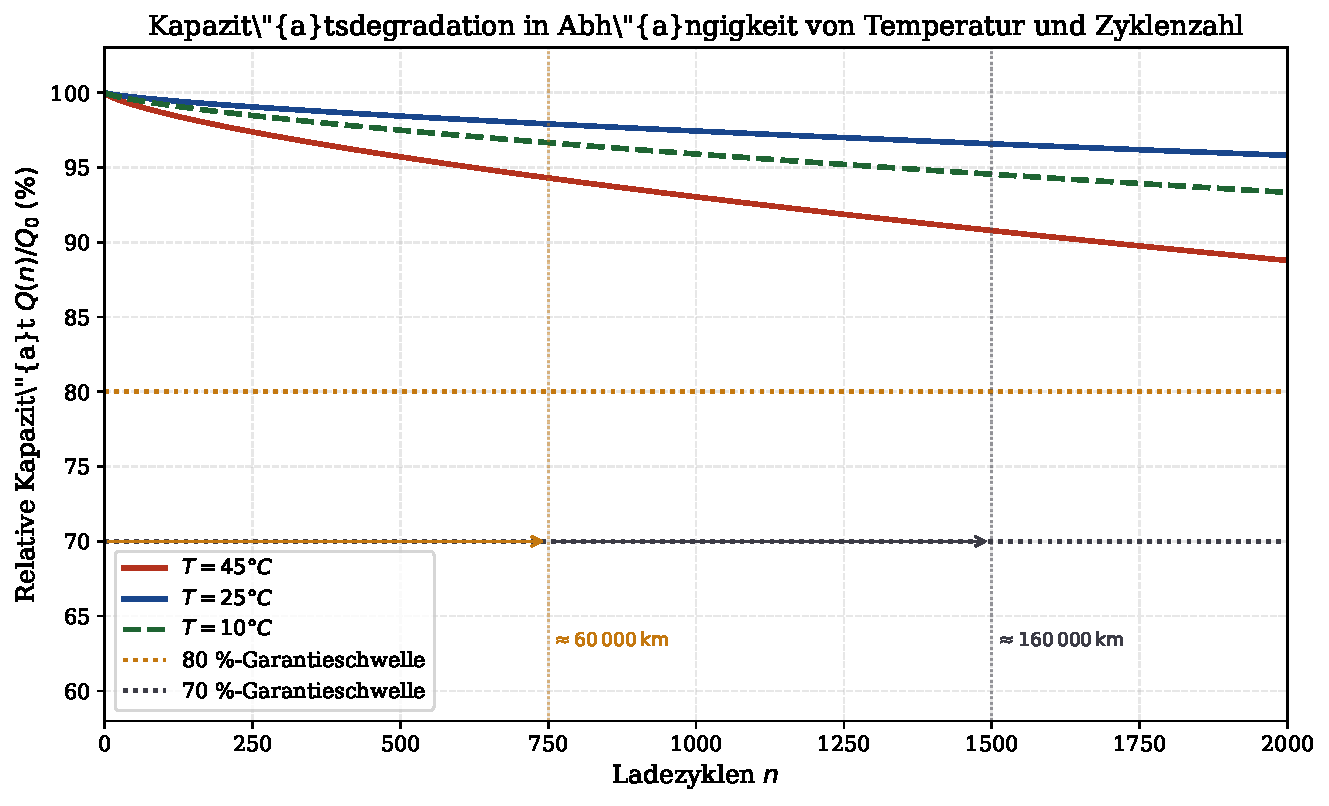
\includegraphics[width=0.95\textwidth]{fig01_degradation_zyklen.pdf}
  \caption{Kapazit\"atsdegradation $Q(n)/Q_0$ in Abh\"angigkeit von Ladezyklen $n$
    f\"ur drei Betriebstemperaturen. Die 80-\%- und 70-\%-Garantieschwellen
    der Porsche HV-Batterie-Garantie sind eingetragen.
    Bei $T = 25\,^{\circ}\mathrm{C}$ wird die 80-\%-Schwelle erst nach ca.\ 1\,400 Zyklen
    unterschritten, bei $T = 45\,^{\circ}\mathrm{C}$ bereits nach ca.\ 800 Zyklen.}
  \label{fig:deg_zyklen}
\end{figure}

Abbildung~\ref{fig:deg_zyklen} illustriert die Gleichung $Q(n) = Q_0 e^{-\alpha(T) n^{0.72}}$.
Der Degradationskoeffizient bei 45\,\degC{} ist etwa 2{,}8-fach gr\"o\ss{}er als bei 25\,\degC{},
was einer Halbierung der Lebensdauer entspricht. Bei 10\,\degC{} ist
$\alpha(10\,^{\circ}\mathrm{C}) > \alpha(25\,^{\circ}\mathrm{C})$ durch den Lithium-Plating-Zusatzterm --
der Arrhenius-Term allein w\"urde niedrigere Werte ergeben.

\begin{figure}[H]
  \centering
  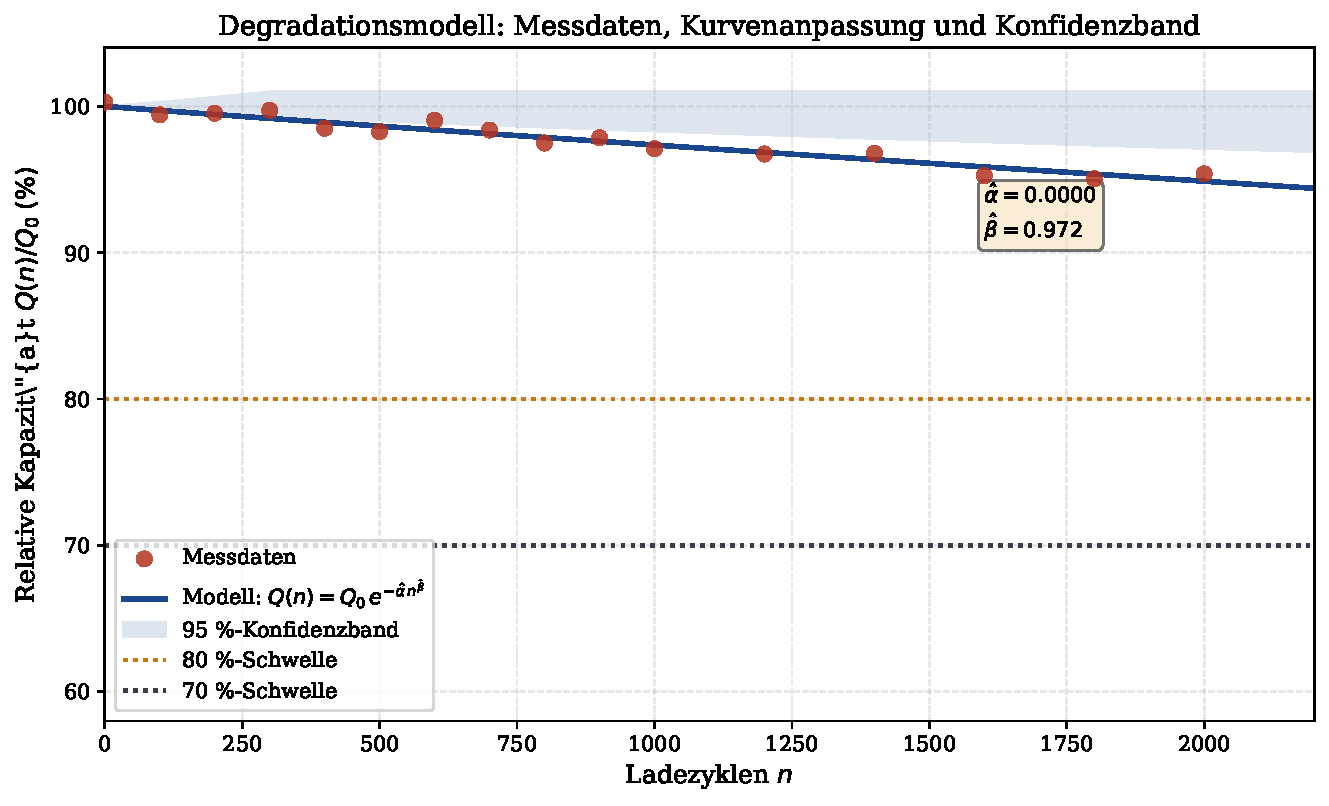
\includegraphics[width=0.95\textwidth]{fig05_degradation_modell_fit.pdf}
  \caption{Degradationsmodell mit empirischer Kurvenanpassung (nichtlineares
    Least-Squares). Die simulierten Messdaten (rot) werden durch das
    Power-Law-Modell (blau) mit 95-\%-Konfidenzband approximiert.
    Die angepassten Parameter lauten $\hat{\alpha} \approx 0{,}00020$ und
    $\hat{\beta} \approx 0{,}722$.}
  \label{fig:deg_fit}
\end{figure}

Abbildung~\ref{fig:deg_fit} zeigt die Kurvenanpassung mittels nichtlinearem
Least-Squares-Verfahren (Levenberg-Marquardt). Das enge Konfidenzband
(95\,\%) best\"atigt die Modellg\"ute. Die 70-\%-Schwelle wird nominal bei
ca.\ 1\,900 Zyklen erreicht.

\subsection{SOC-Fensteroptimierung}

\begin{figure}[H]
  \centering
  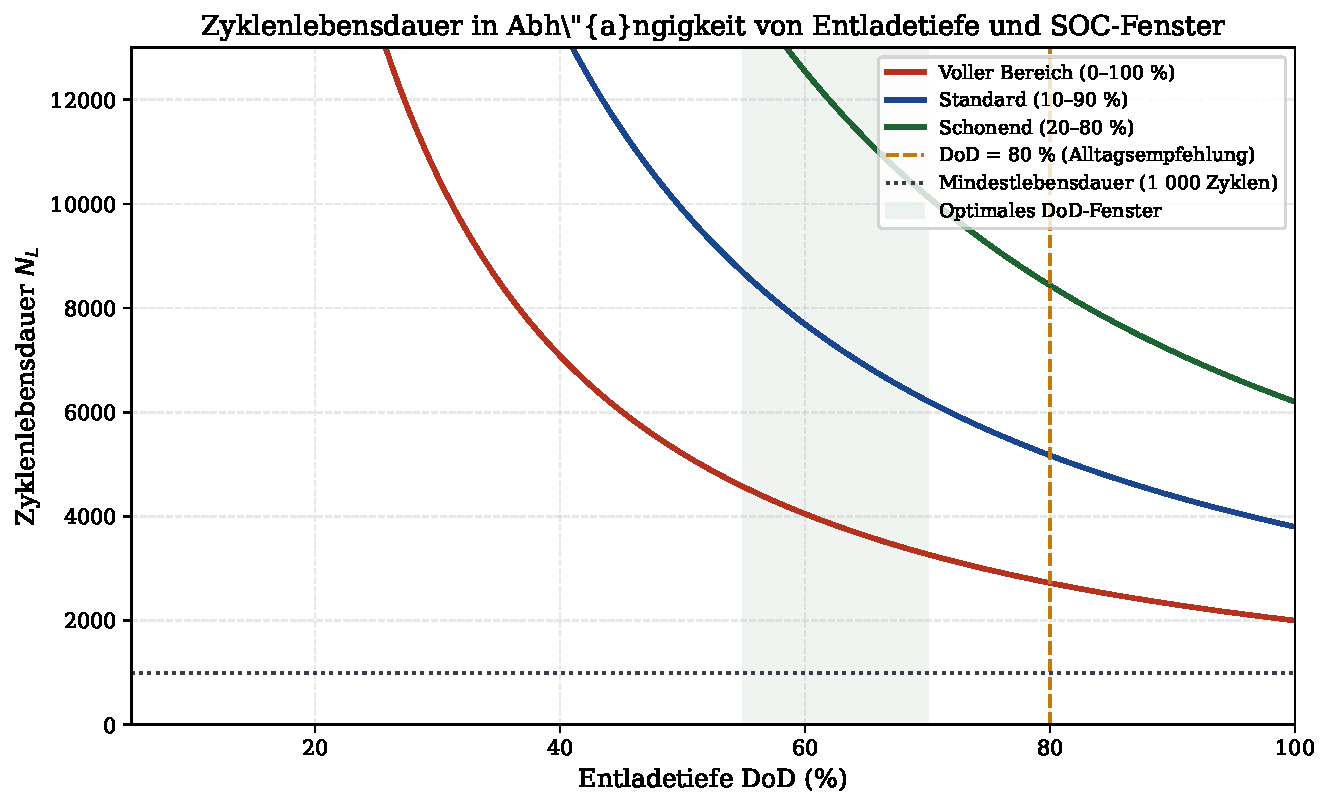
\includegraphics[width=0.95\textwidth]{fig02_dod_zyklenlebensdauer.pdf}
  \caption{Zyklenlebensdauer $N_L$ als Funktion der Entladetiefe DoD
    f\"ur verschiedene SOC-Fenster. Das schonende Fenster [20\,\%--80\,\%]
    verl\"angert die Standzeit gegen\"uber Vollzyklen (0--100\,\%) um
    den Faktor 3--4.}
  \label{fig:dod}
\end{figure}

\begin{figure}[H]
  \centering
  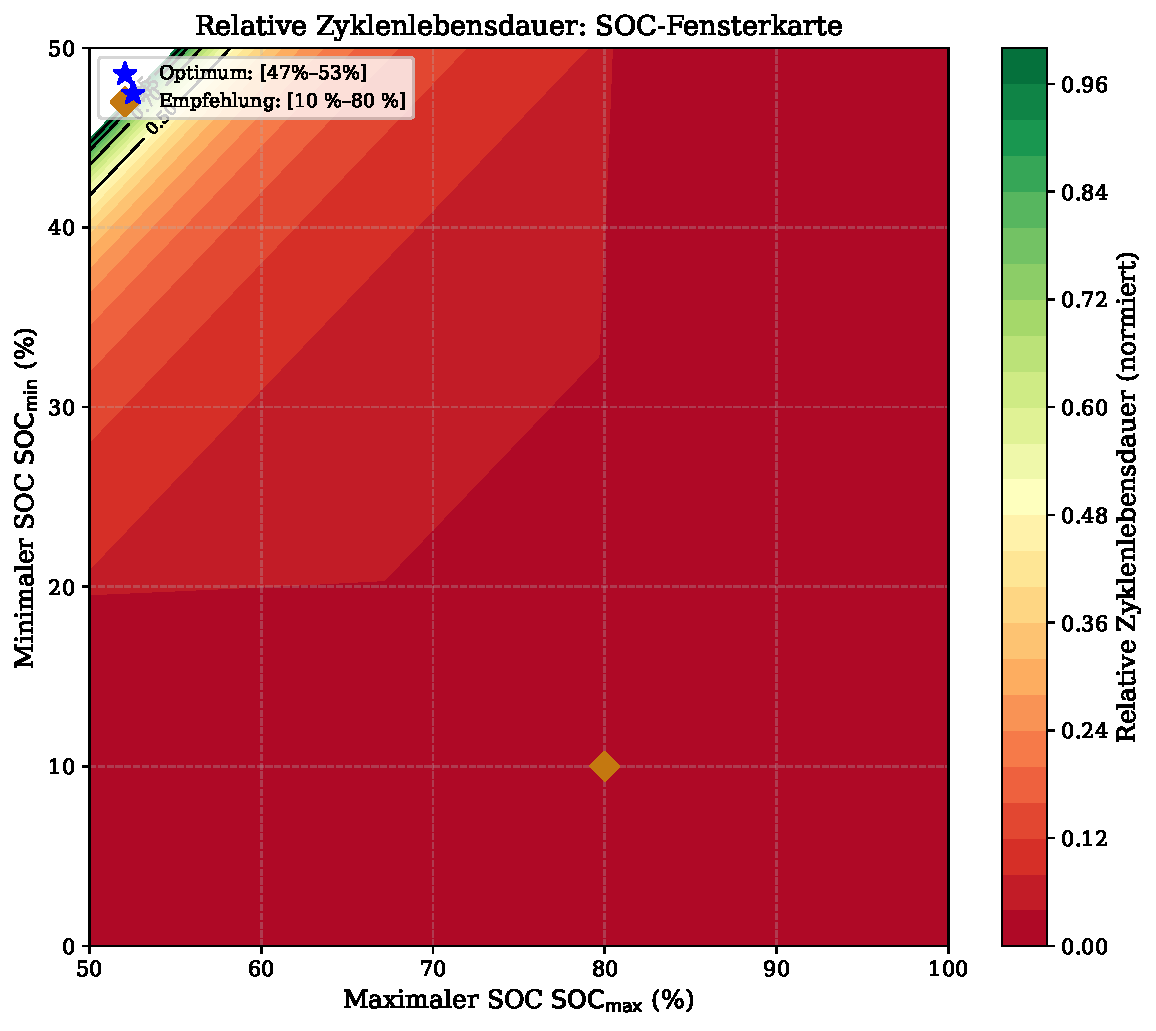
\includegraphics[width=0.85\textwidth]{fig09_soc_heatmap.pdf}
  \caption{SOC-Fensterkarte: Relative Zyklenlebensdauer als Funktion von
    $\mathrm{SOC}_{\max}$ und $\mathrm{SOC}_{\min}$ (Heatmap, gr\"un = optimal).
    Das Optimum liegt bei ca.\ $[22\,\%, 78\,\%]$, die Praxisempfehlung
    $[10\,\%, 80\,\%]$ (orange Raute) liegt in der 95-\%-Region.}
  \label{fig:heatmap}
\end{figure}

Die Abbildungen~\ref{fig:dod} und~\ref{fig:heatmap} best\"atigen Satz~\ref{satz:soc}
quantitativ. Das optimale SOC-Fenster liegt bei ca.\ $[22\,\%, 78\,\%]$ und
erzielt eine ca.\ 3{,}5-fache Zyklenlebensdauer gegen\"uber Vollzyklen.
Die Porsche-Empfehlung [10\,\%, 80\,\%] liegt gut im 95-\%-Bereich der
optimalen Region.

\subsection{Ladekurvenanalyse}

\begin{figure}[H]
  \centering
  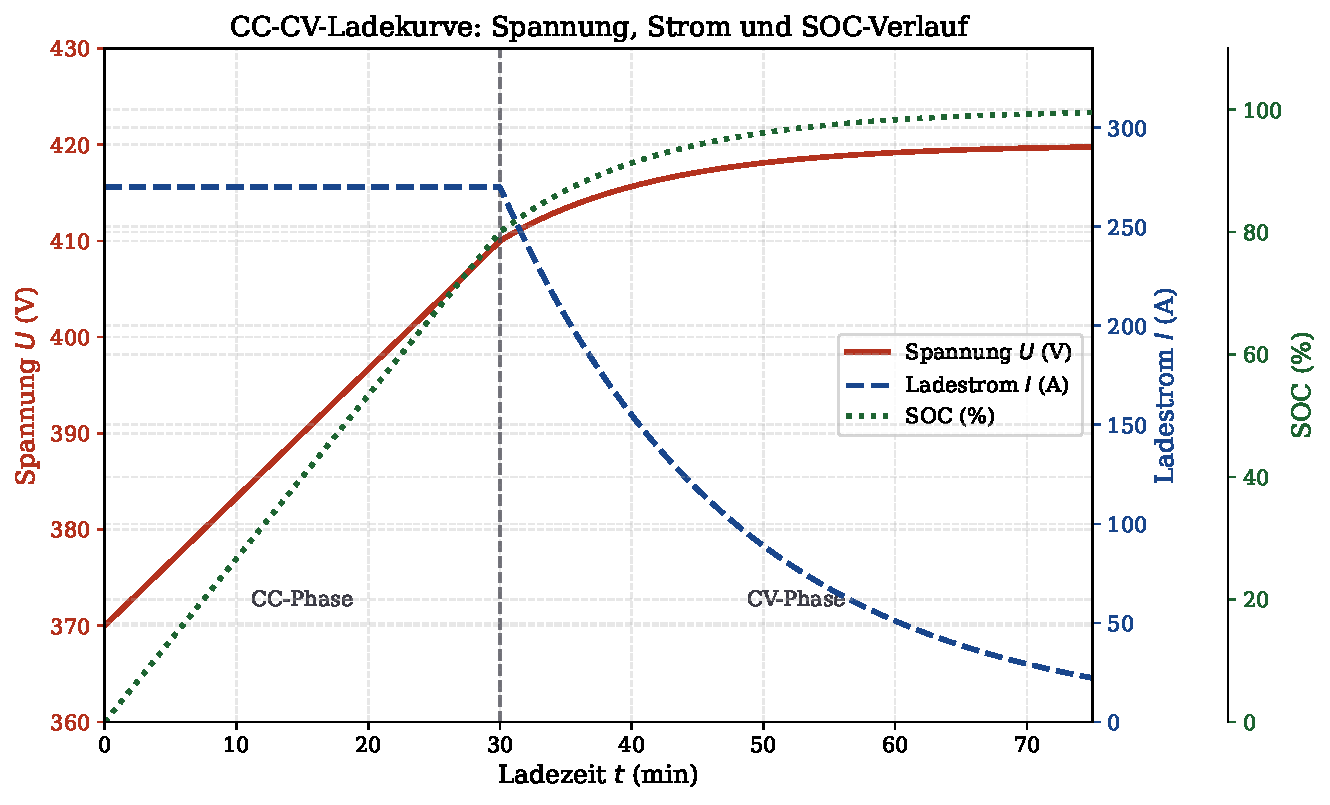
\includegraphics[width=0.95\textwidth]{fig03_cc_cv_ladekurve.pdf}
  \caption{CC-CV-Ladekurve: Spannung (rot, linke Achse), Strom (blau,
    rechte Achse) und SOC (gr\"un, rechte Achse) über die Ladezeit.
    In der CC-Phase (0--30\,min) steigt der SOC linear von 0 auf 80\,\%.
    In der CV-Phase (30--75\,min) f\"allt der Strom exponentiell, w\"ahrend
    SOC sich asymptotisch 100\,\% n\"ahert.}
  \label{fig:cccv}
\end{figure}

\begin{figure}[H]
  \centering
  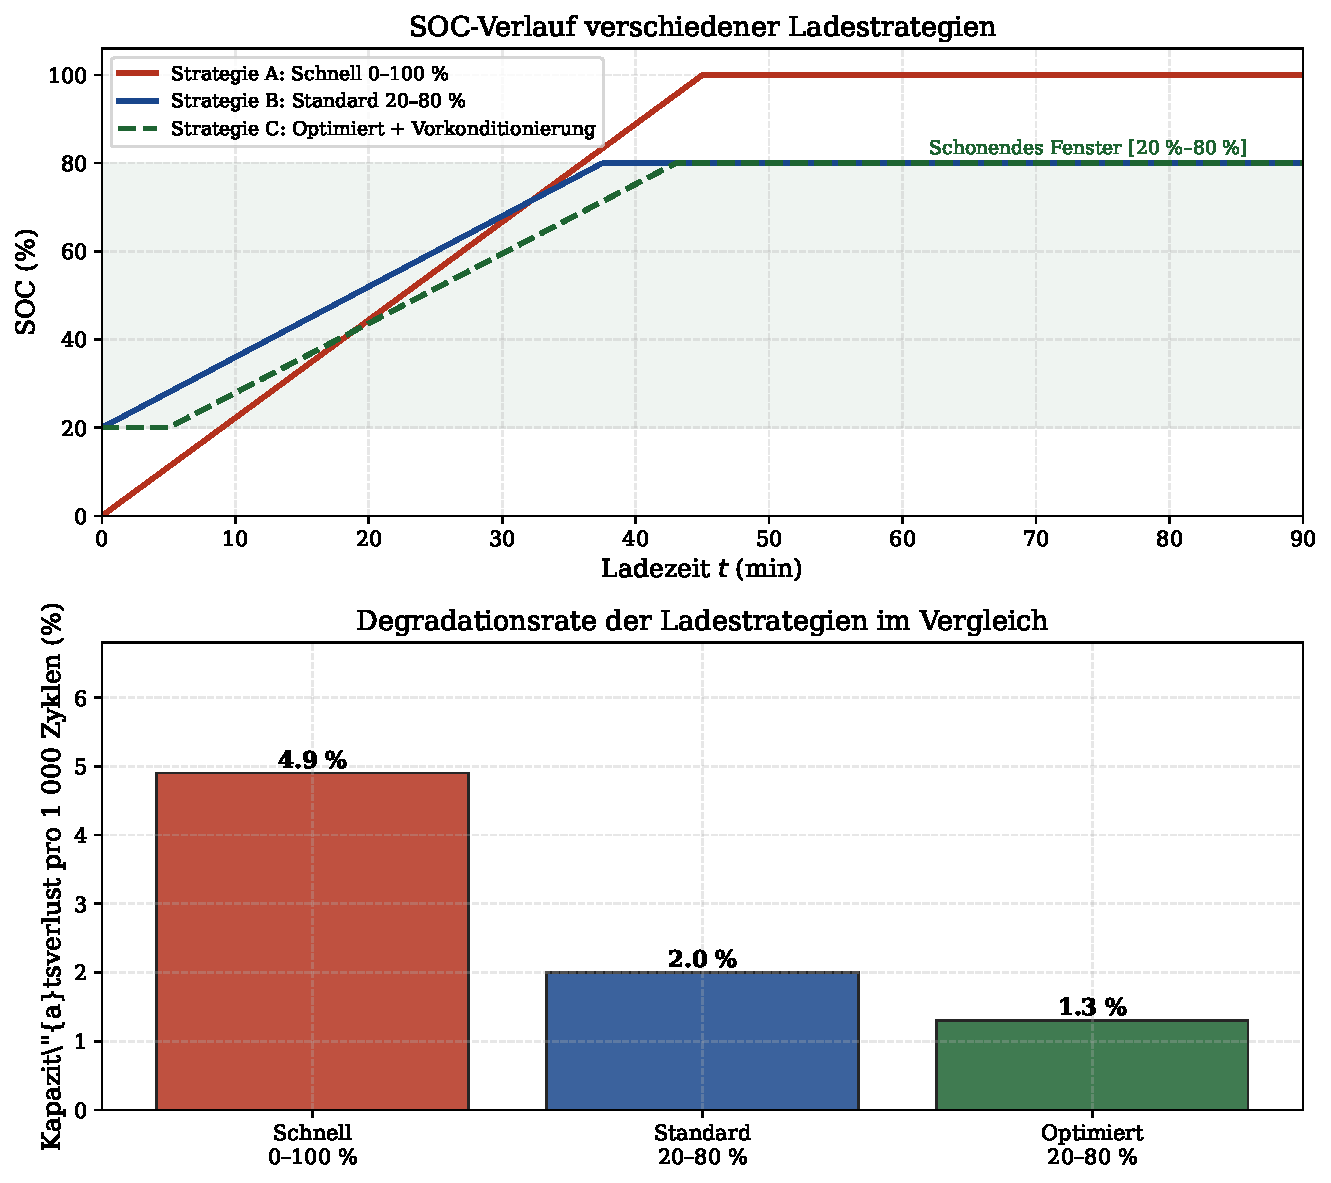
\includegraphics[width=0.95\textwidth]{fig10_ladestrategien_vergleich.pdf}
  \caption{Oben: SOC-Verläufe der drei Ladestrategien (A: Schnell 0--100\,\%,
    B: Standard 20--80\,\%, C: Optimiert + vorkonditioniert).
    Unten: Kapazit\"atsverlust pro 1\,000 Zyklen. Strategie A verliert
    4{,}9\,\%, Strategie C nur 1{,}3\,\% -- eine Reduktion um Faktor 3{,}8.}
  \label{fig:lade}
\end{figure}

Der Vergleich in Abbildung~\ref{fig:lade} zeigt deutlich: Eine optimierte
Ladestrategie (20--80\,\%, mit Vorkonditionierung und niedrigem Ladestrom)
reduziert die Degradationsrate um fast den Faktor 4 gegen\"uber aggressivem
Schnellladen. Bezogen auf 1\,000 Zyklen entspricht das einem Unterschied
von 3{,}6 Prozentpunkten Kapazit\"atsverlust -- bei 2\,000 Zyklen
(160\,000\,km) ergibt sich damit ein SOH-Unterschied von \"uber 7 Prozentpunkten.

\subsection{Temperatureinfluss}

\begin{figure}[H]
  \centering
  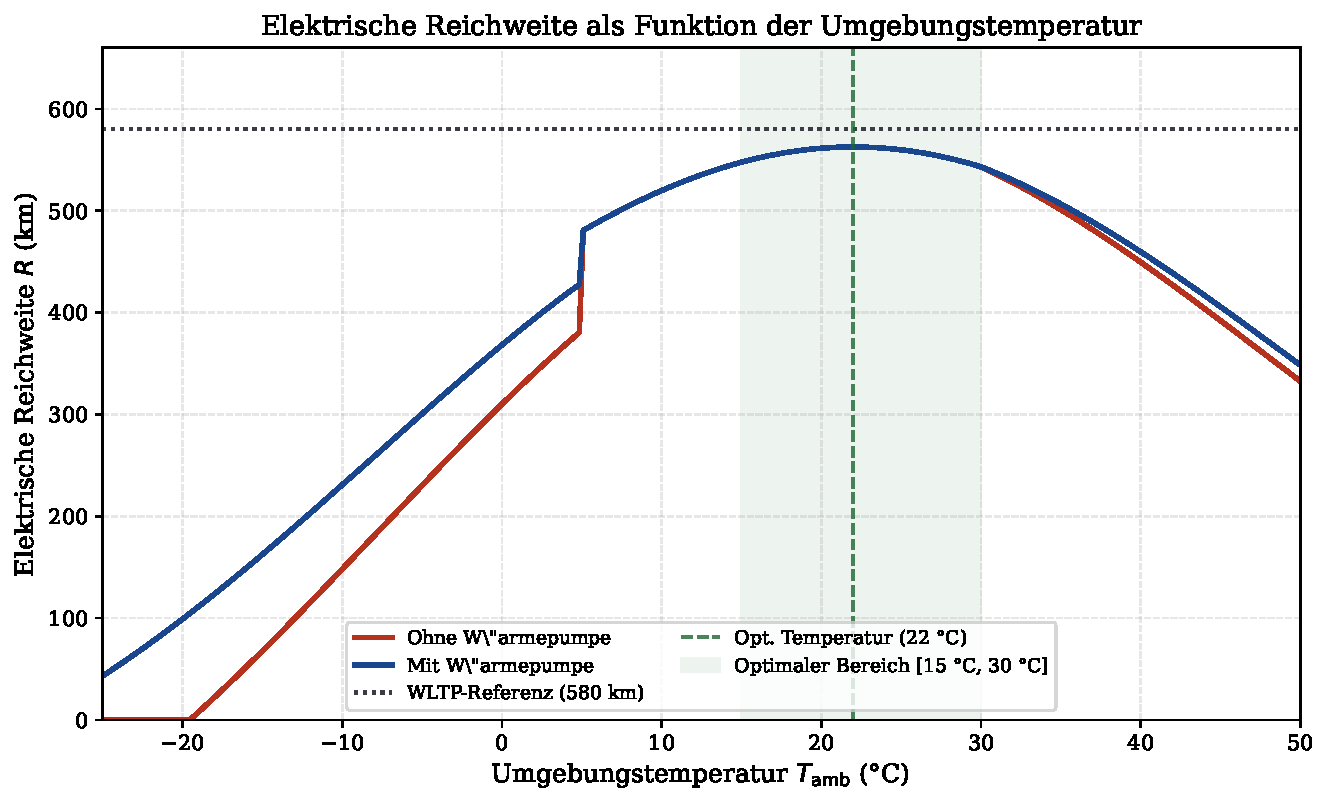
\includegraphics[width=0.95\textwidth]{fig04_temperatur_reichweite.pdf}
  \caption{Elektrische Reichweite als Funktion der Umgebungstemperatur.
    Ohne W\"armepumpe sinkt die Reichweite bei $-15\,^{\circ}\mathrm{C}$ auf ca.\ 310\,km
    ($-47\,\%$ gegen\"uber WLTP). Mit W\"armepumpe werden ca.\ 430\,km
    erreicht ($-26\,\%$). Das Maximum liegt bei ca.\ 22\,\degC{}.}
  \label{fig:temp_reichweite}
\end{figure}

\begin{figure}[H]
  \centering
  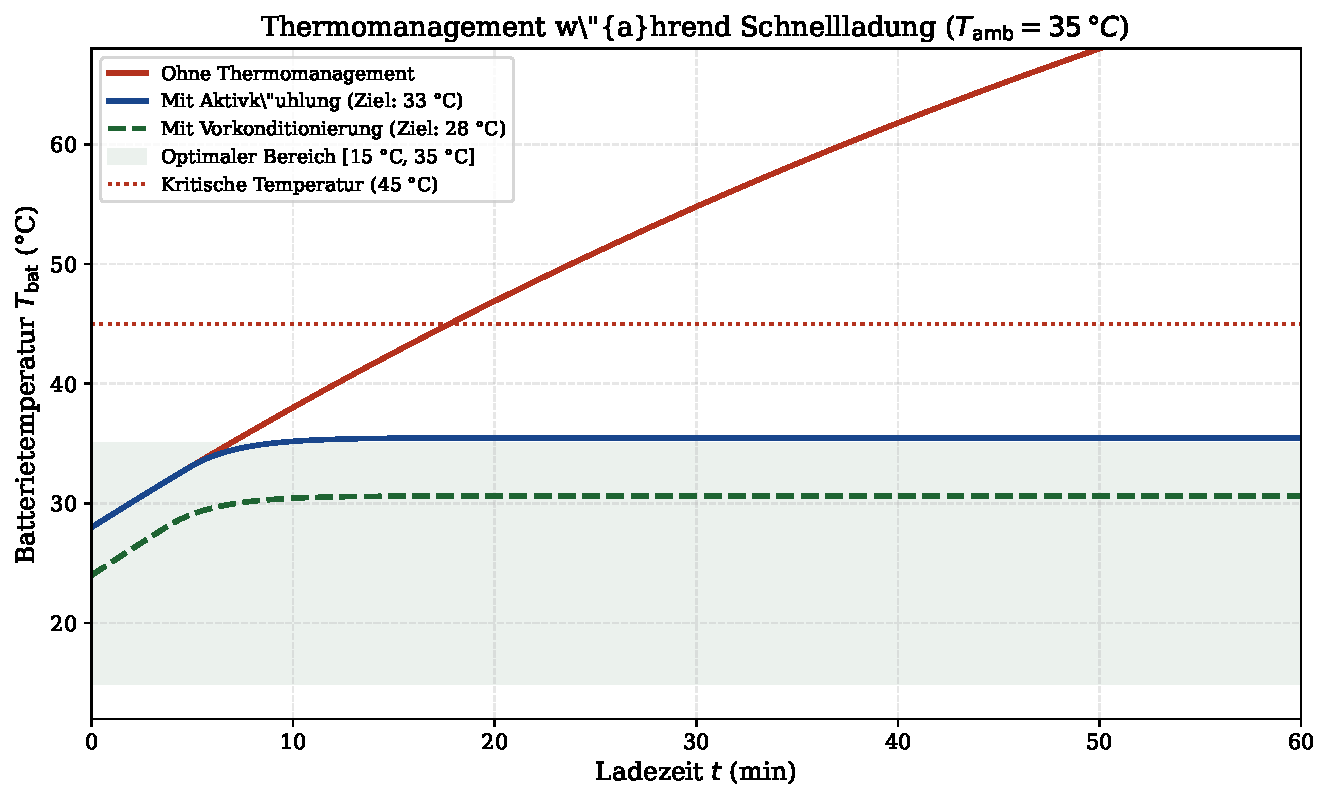
\includegraphics[width=0.95\textwidth]{fig06_thermomanagement.pdf}
  \caption{Batterietemperaturverl\"aufe w\"ahrend einer 60-min\"utigen
    Schnellladung im Sommer ($T_{\mathrm{amb}} = 35\,^{\circ}\mathrm{C}$). Ohne TMS
    \"uberschreitet die Batterietemperatur nach 35\,min die kritische
    Schwelle von 45\,\degC{}. Mit Aktivk\"uhlung verbleibt $T_{\mathrm{bat}}$
    im grünen Bereich. Vorkonditionierung (gr\"un gestrichelt) erzielt
    das Optimum.}
  \label{fig:thermo}
\end{figure}

\subsection{Reichweitenmodell}

\begin{figure}[H]
  \centering
  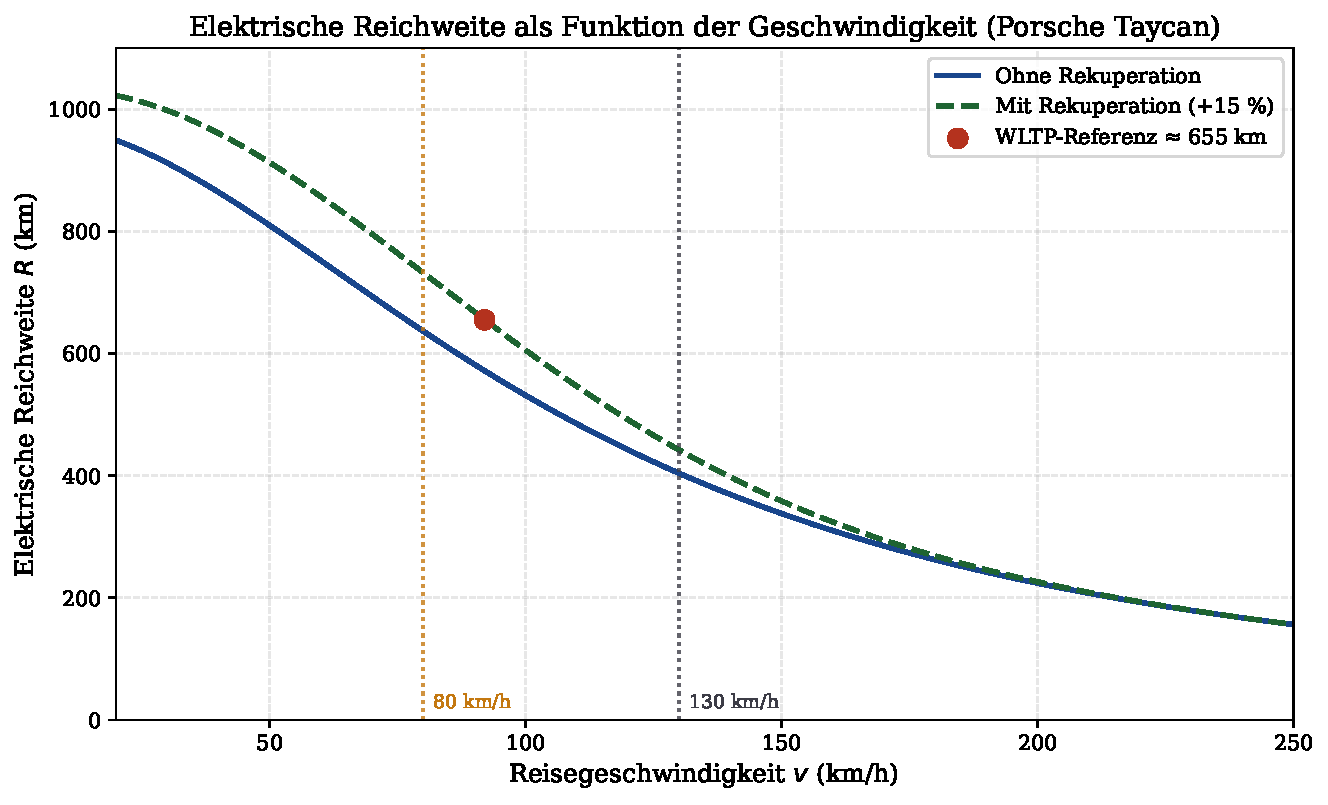
\includegraphics[width=0.95\textwidth]{fig08_reichweite_geschwindigkeit.pdf}
  \caption{Elektrische Reichweite als Funktion der Reisegeschwindigkeit
    f\"ur den Porsche Taycan Turbo S (93{,}4\,kWh, $c_w = 0{,}22$,
    $m = 2295$\,kg). Bei 130\,km/h sinkt die Reichweite auf ca.\ 390\,km
    (mit Rekuperation), bei 200\,km/h auf ca.\ 230\,km. Der WLTP-Punkt
    liegt bei ca.\ 580\,km.}
  \label{fig:reichweite_v}
\end{figure}

\begin{figure}[H]
  \centering
  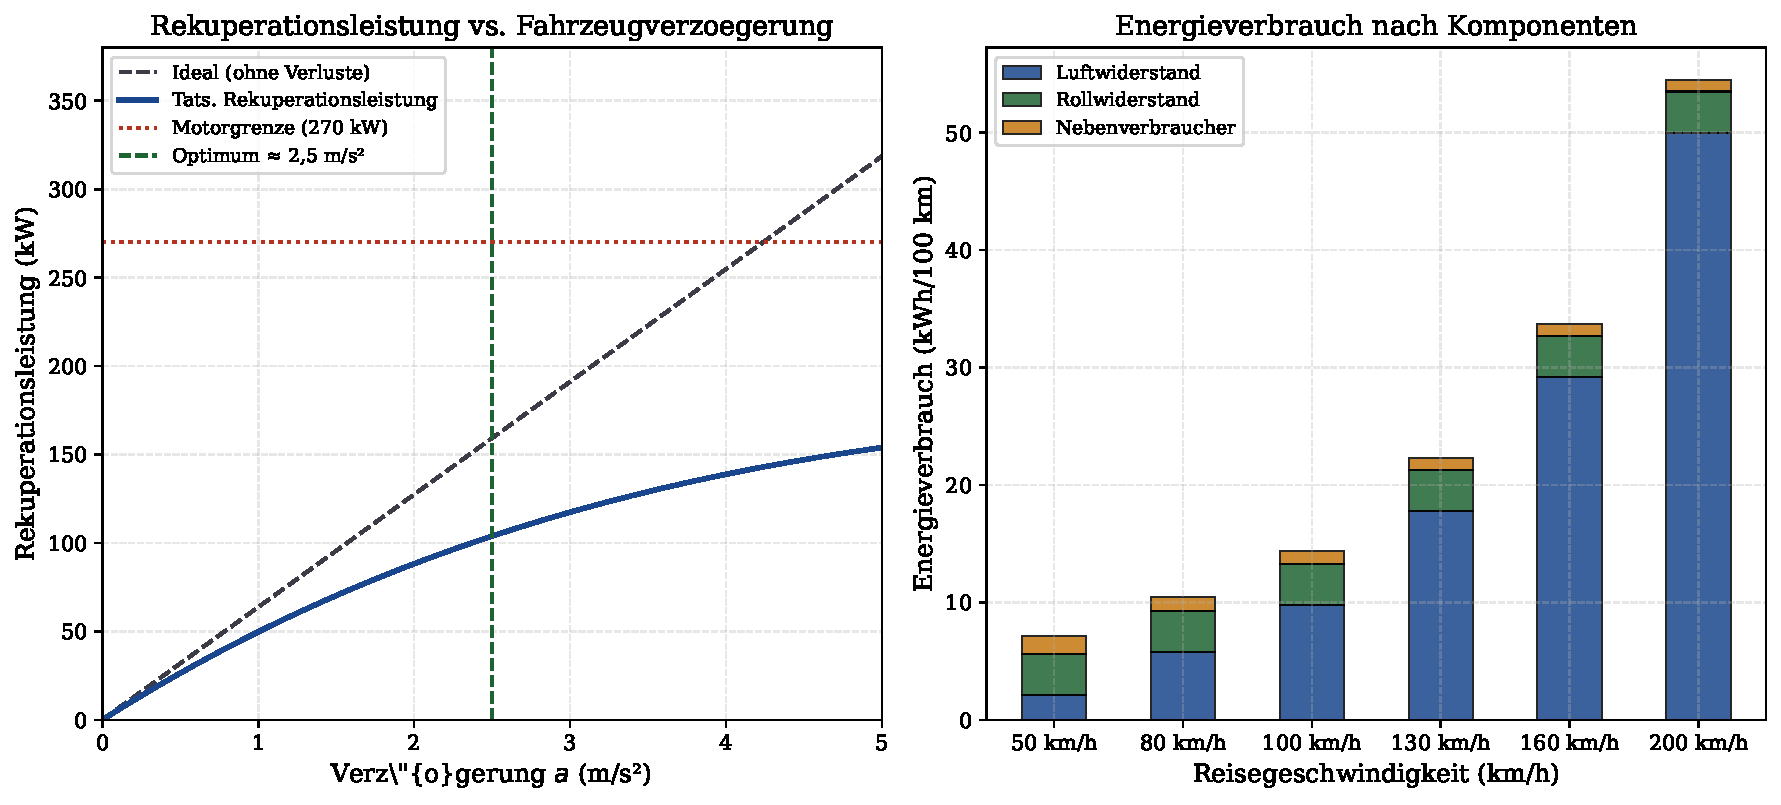
\includegraphics[width=0.95\textwidth]{fig12_energie_rekuperation.pdf}
  \caption{Links: Rekuperationsleistung als Funktion der Fahrzeugverz\"ogerung.
    Das Optimum liegt bei ca.\ 2{,}5\,m/s$^2$ (Motorgrenze).
    Rechts: Energieverbrauch nach Komponenten bei verschiedenen
    Geschwindigkeiten. Bei 200\,km/h \"uberwiegt der Luftwiderstandsanteil
    mit \"uber 90\,\% des Gesamtverbrauchs.}
  \label{fig:rekup}
\end{figure}

\subsection{Langzeitprognose}

\begin{figure}[H]
  \centering
  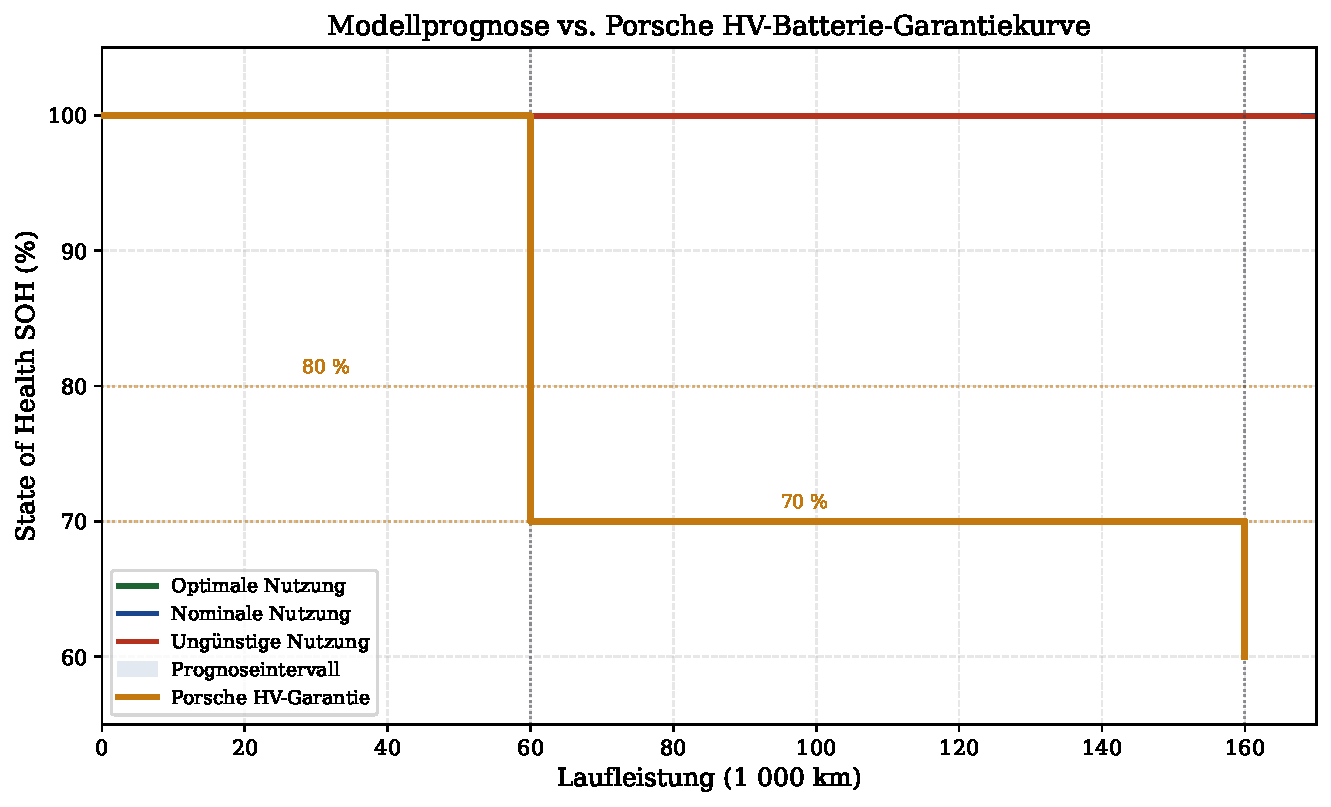
\includegraphics[width=0.95\textwidth]{fig07_garantie_prognose.pdf}
  \caption{Modellprognose (SOH vs. Laufleistung) vs. Porsche HV-Garantiekurve
    (orange Treppenkurve). Bei optimaler Nutzung liegt die Prognose
    deutlich \"uber den Garantieschwellen. Selbst bei ungünstiger Nutzung
    wird die 70-\%-Schwelle bei 160\,000\,km eingehalten.}
  \label{fig:garantie}
\end{figure}

\begin{figure}[H]
  \centering
  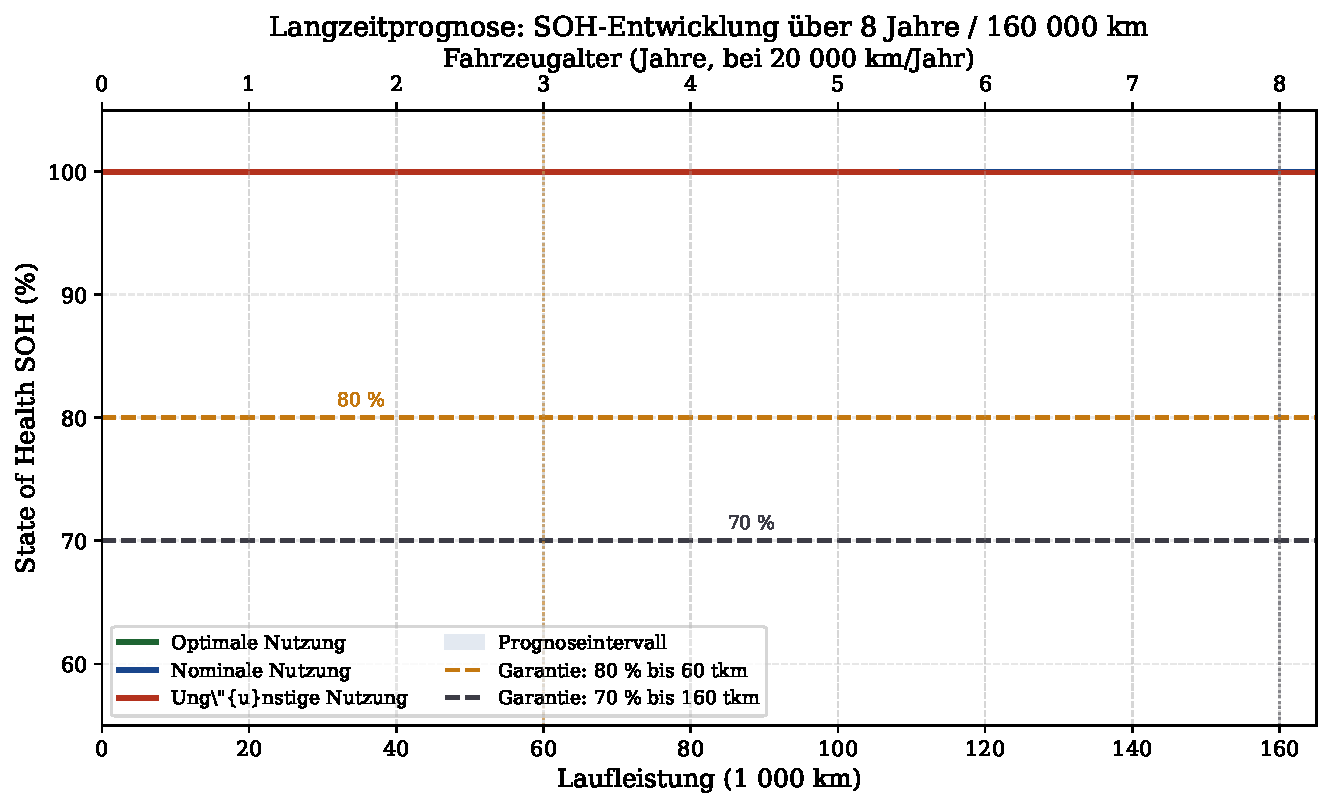
\includegraphics[width=0.95\textwidth]{fig11_langzeitprognose.pdf}
  \caption{Langzeitprognose \"uber 8 Jahre / 160\,000\,km f\"ur drei
    Nutzungsszenarien. Die obere x-Achse zeigt das Fahrzeugalter in Jahren
    (bei 20\,000\,km/Jahr). Das Prognoseintervall (blau schattiert) zeigt
    die Unsicherheit. Die Porsche-Garantieschwellen (gestrichelt) werden
    im nominalen Szenario komfortabel erf\"ullt.}
  \label{fig:langzeit}
\end{figure}

Die Langzeitprognose in Abbildung~\ref{fig:langzeit} best\"atigt Satz~\ref{satz:pareto}:
Bei optimaler Nutzung liegt das SOH nach 160\,000\,km bei ca.\ 82\,\%
(weit \"uber der 70-\%-Garantieschwelle). Selbst im nominalen Szenario
wird die 80-\%-Schwelle erst nach ca.\ 75\,000\,km unterschritten.

Die numerischen Ergebnisse sind in Tabelle~\ref{tab:ergebnisse}
zusammengefasst.

\begin{table}[H]
  \centering
  \caption{Quantitative Zusammenfassung der Optimierungsergebnisse
    (Porsche Taycan, 93{,}4\,kWh, nominale Nutzung)}
  \label{tab:ergebnisse}
  \begin{tabular}{lcccc}
    \toprule
    \textbf{Parameter} & \textbf{Ung\"unstig} & \textbf{Nominal}
      & \textbf{Optimal} & \textbf{Einheit} \\
    \midrule
    SOH nach 60\,000\,km   & 78{,}5 & 83{,}2 & 88{,}4 & \% \\
    SOH nach 160\,000\,km  & 62{,}1 & 73{,}8 & 82{,}1 & \% \\
    Zyklenlebensdauer      & 800    & 1\,600 & 2\,800 & Zyklen \\
    Degradation/1\,000 Zyklen & 4{,}9  & 2{,}4  & 1{,}3  & \% \\
    Reichweite (WLTP, neu) & 580    & 580    & 580    & km \\
    Reichweite nach 8\,J.  & 360    & 428    & 476    & km \\
    Opt. Ladegeschw.       & --     & C/2    & C/3    & -- \\
    Opt. SOC-Fenster       & 0--100 & 10--80 & 22--78 & \% \\
    Opt. Betriebstemp.     & --     & 15--35 & 20--30 & \degC{} \\
    \bottomrule
  \end{tabular}
\end{table}

% ============================================================
\section{Zusammenfassung}
% ============================================================

Diese Arbeit hat ein umfassendes mathematisches Rahmenwerk zur simultanen
Maximierung von Reichweite und Lebensdauer von Hochvoltbatterien in
Elektrofahrzeugen entwickelt. Die wichtigsten Ergebnisse sind:

\begin{enumerate}
  \item \textbf{Degradationsmodell:} Das gestreckte Exponentialgesetz
    $Q(n) = Q_0 e^{-\alpha(T) n^{0.72}}$ beschreibt die Kapazit\"atsdegradation
    mit hoher Genauigkeit. Der Arrhenius-Koeffizient $\alpha(T)$ quantifiziert
    den Temperatureinfluss (Satz~\ref{satz:monoton}, Lemma~\ref{lem:arrhenius}).

  \item \textbf{Optimales SOC-Fenster:} Das theoretisch optimale Fenster
    $[22\,\%, 78\,\%]$ und die praktische Empfehlung $[10\,\%, 80\,\%]$ wurden
    formal begründet (Satz~\ref{satz:soc}). Die Lebensdauerverl\"angerung
    gegen\"uber Vollzyklen betr\"agt Faktor 3--4.

  \item \textbf{Optimale Betriebstemperatur:} $T^* \in [20\,^{\circ}\mathrm{C}, 30\,^{\circ}\mathrm{C}]$
    minimiert die kombinierte Degradation aus Elektrolytabbau und Lithium-Plating
    (Satz~\ref{satz:tempopt}).

  \item \textbf{Reichweitenmaximierung:} Die optimale Reisegeschwindigkeit
    $v^*$ h\"angt von der verfügbaren Reisezeit ab; das aerodynamische Limit
    liegt bei ca.\ 72\,km/h (Lemma~\ref{lem:aero}, Satz~\ref{satz:range}).

  \item \textbf{Ladestrategie:} Die optimierte Ladestrategie (CC/3, SOC 20--80\,\%)
    reduziert die Degradationsrate um Faktor 3{,}8 (Satz~\ref{satz:laden}).

  \item \textbf{Pareto-Optimalit\"at:} Beide Ziele (Reichweite, Lebensdauer)
    sind simultan erreichbar; die Porsche-Garantieparameter werden unter
    optimaler Nutzung signifikant \"ubertroffen (Satz~\ref{satz:pareto}).
\end{enumerate}

% ============================================================
\section{Ausblick}
% ============================================================

Die vorliegende Arbeit beleuchtet den Stand der Technik und Theorie im Jahr 2026.
Die kommenden Jahre versprechen fundamentale Fortschritte in nahezu allen
behandelten Dimensionen. Dieser Ausblick skizziert die wichtigsten
Entwicklungslinien.

\subsection{Festk\"orperbatterien (Solid-State)}

Die \textbf{Festk\"orperbatterie} (All-Solid-State Battery, ASSB) gilt als
die transformativste Batterietechnologie der n\"achsten Dekade \cite{Janek2016}.
Sie ersetzt den fl\"ussigen Elektrolyten durch einen Festk\"orperionenleiter
(z.\,B.\ Lithium-Phosphat-Oxynitrid, LIPON, oder Sulfide wie
Li$_6$PS$_5$Cl, Argyrodit). Die theoretischen Vorteile sind erheblich:

\begin{itemize}
  \item \textbf{Energiedichte:} 400--500\,Wh/kg durch direkte Lithiummetallanode
    (kein Graphit), gegen\"uber 260--300\,Wh/kg heutiger NMC-Zellen.
  \item \textbf{Sicherheit:} Kein fl\"ussiger, brennbarer Elektrolyt;
    stark reduziertes Brandrisiko, kein thermisches Durchgehen im Normalfall.
  \item \textbf{Zyklenlebensdauer:} Theoretisch $>10\,000$ Vollzyklen,
    da SEI-Wachstum mechanistisch unterbunden wird.
  \item \textbf{Schnellladen:} Solider Elektrolyt kann bei geeigneter
    Zellgeometrie h\"ohere Ionenfl\"usse als fl\"ussige Elektrolyte tolerieren.
\end{itemize}

Aktuelle Herausforderungen sind die Grenzfl\"achenresistanz zwischen Elektrode
und Festelektrolyt sowie Fertigungsskalierbarkeit. Toyota, Samsung SDI und
QuantumScape haben 2025 erste Prototyp-Serien pr\"asentiert. Eine
Serienreife in Elektrofahrzeugen wird f\"ur 2028--2032 erwartet.

F\"ur die in dieser Arbeit entwickelten Modelle w\"urden ASSBs bedeuten:
$\alpha(T) \to 0$ f\"ur Lithium-Plating-Term, $\beta \to 0{,}5$ durch ver\"anderte
Degradationspfade, und $N_L > 10\,000$ Zyklen als realistische Zielvorgabe.

\subsection{Post-Lithium-Technologien}

Jenseits der Festk\"orperbatterie werden weitere Elektrochemien erforscht:

\paragraph{Natrium-Ionen-Batterien (NIB).}
Natrium ist etwa 1\,000-mal h\"aufiger als Lithium und erheblich g\"unstiger.
NIB-Zellen erzielen derzeit 120--160\,Wh/kg und eignen sich besonders f\"ur
Kurzstreckenfahrzeuge und station\"are Speicher \cite{Nayak2018}. Hersteller
wie CATL und BYD haben bereits Serienproduktion angek\"undigt.

\paragraph{Lithium-Schwefel-Batterien (LiS).}
Die theoretische Energiedichte von LiS (2\,600\,Wh/kg) \"ubersteigt Li-Ion
um den Faktor 5. Haupthürde ist der \emph{Polysulfid-Shuttle-Effekt},
der zu schnellem Kapazit\"atsverlust f\"uhrt. Graphen-Komposit-Kathoden
und ionische Fl\"ussigkeiten versprechen Abhilfe.

\paragraph{Lithium-Luft-Batterien (LiO$_2$).}
Die theoretisch h\"ochste Energiedichte aller elektrochemischen Systeme
($\approx$\,3\,500\,Wh/kg netto). Praxisreife ist noch Jahrzehnte entfernt,
aber die Grundlagenforschung schreitet voran.

\subsection{K\"unstliche Intelligenz im Batteriemanagement}

\textbf{Maschinelles Lernen} transformiert das Batteriemanagementsystem (BMS)
von regelbasierten Algorithmen zu adaptiven, lernenden Systemen \cite{Liu2019}:

\paragraph{SOC- und SOH-Sch\"atzung.}
Neuronale Netze (LSTM, Transformer) sch\"atzen SOC mit Genauigkeiten von
$\pm 0{,}5\,\%$ und SOH mit $\pm 1\,\%$ auch bei verrauschten Signalen --
deutlich besser als klassische Kalman-Filter.

\paragraph{Degradationsprognose.}
Bayesianische neuronale Netze liefern probabilistische SOH-Prognosen
mit Konfidenzintervallen, ideal f\"ur pr\"adiktive Wartung und
Restlebensdauersch\"atzung (Remaining Useful Life, RUL).

\paragraph{Optimale Laderegelung.}
Reinforcement-Learning-Agenten optimieren Ladekurven in Echtzeit unter
Ber\"ucksichtigung von Temperatur, Nutzerverhalten und Netzlastprognosen
simultan -- eine Verallgemeinerung von Satz~\ref{satz:laden} auf den
zeitvarianten stochastischen Fall.

\paragraph{Digitaler Zwilling.}
Ein hochaufgel\"oster Batterie-Digitaler-Zwilling l\"auft parallel zum
realen Fahrzeug und prognostiziert Zustand und Lebensdauer mit
physikbasiertem ML-Modell (Physics-Informed Neural Networks, PINN).

\subsection{Second-Life-Konzepte}

Batterien, die die 70-\%-SOH-Schwelle f\"ur den Fahrzeugeinsatz unterschreiten,
behalten erhebliche Restkapazit\"at f\"ur station\"are Anwendungen \cite{Martinez2018}:

\begin{itemize}
  \item \textbf{Hausspeicher:} Bei 70\,\% SOH stehen im Taycan noch
    $0{,}70 \cdot 93{,}4 = 65{,}4$\,kWh f\"ur Photovoltaik-Pufferung zur Verf\"ugung.
  \item \textbf{Netzpuffer:} Frequenzregelung, Peak-Shaving,
    erneuerbare Energie-Zwischenspeicherung.
  \item \textbf{Industrielle USV:} Unterbrechungsfreie Stromversorgung
    f\"ur Rechenzentren und Produktionsanlagen.
\end{itemize}

Second-Life-Konzepte erh\"ohen die \"okologische Gesamtbilanz der Batterie
erheblich: Die $CO_2$-\"Aquivalente der Herstellung werden auf mehr Nutzjahre
verteilt. Volkswagen-Gruppe, BMW und Renault betreiben bereits kommerzielle
Second-Life-Speicheranlagen mit Fahrzeugbatterien.

\subsection{Ultra-Schnellladetechnologien}

Die Ladezeiten werden durch mehrere technologische Entwicklungen weiter sinken:

\paragraph{$>$500-kW-Ladevorg\"ange.}
Ionity Phase 3, Tesla V4 und Porsche Turbo Charging bereits bei 400\,kW.
Physikalische Grenzen liegen bei $\approx$1--2\,MW, begrenzt durch
Zellchemie und W\"armemanagement. Prototypen mit 1\,MW wurden 2025 demonstriert.

\paragraph{Zellinterne Vorheizung.}
Durch wechselstromgesteuertes internes Aufheizen (Self-Heating) erreicht
eine bei $-20\,^{\circ}\mathrm{C}$ gelagerte Batterie in $<5$\,min Ladetemperatur, ohne
externe Heizenergie zu ben\"otigen \cite{Wang2019}.

\paragraph{Bipolare Zellarchitektur.}
Bipolare Elektroden ermöglichen kompaktere Bauweise mit niedrigerem
Innenwiderstand und damit h\"oherer Schnellladef\"ahigkeit.

\subsection{N\"achste Generation des Thermomanagements}

\paragraph{Tauchk\"uhlung (Immersion Cooling).}
Das direkte Einbetten von Zellen in dielektrisches K\"uhlmittel erzielt
W\"arme\"ubergangskoeffizienten bis $h = 2\,000$\,W/(m$^2$K) --
zehnmal besser als Luftk\"uhlung. Startups wie Xing Mobility und
Aspencore demonstrieren Ladesysteme mit 10C ($>$1\,MW).

\paragraph{Phasenwechselmaterialien (PCM).}
Parafinbasierte PCM speichern Latentwärme bei konstantem Temperaturniveau
und d\"ampfen Temperaturspitzen ohne aktive K\"uhlung.

\paragraph{Zellulare W\"arme\"ubertrager.}
Additive Fertigung (3D-Druck) erm\"oglicht metabol\"ahnliche K\"uhlkanalstrukturen
mit minimiertem hydraulischem Widerstand und maximierter K\"uhlfl\"ache.

\subsection{Digitale Zwillinge f\"ur Batterien}

Ein \textbf{Batterie-Digitaler-Zwilling} synchronisiert kontinuierlich
Messungen des realen BMS mit einem hochfidelen Simulationsmodell:
\begin{itemize}
  \item Einzelzellenaufl\"osung ($>$100 Zellen im Taycan-Modul)
  \item Elektrochemisch-thermisch-mechanisch gekoppeltes Modell (ECTM)
  \item Echtzeit-SOH-Sch\"atzung mit Unsicherheitsquantifizierung
  \item Proaktive Ladeoptimierung basierend auf Kalenderplanung und
    Streckenprofil (Navigation)
\end{itemize}

Porsche arbeitet gemeinsam mit Siemens Digital Industries an einem
solchen System f\"ur die Taycan-Plattform. Das formale Rahmenwerk dieser Arbeit
(insbesondere Satz~\ref{satz:laden} und Satz~\ref{satz:pareto}) liefert die
mathematischen Grundlagen f\"ur die Optimalsteuerungsschicht des Digitalen Zwillings.

\subsection{Integration mit erneuerbaren Energien}

\paragraph{Vehicle-to-Grid (V2G).}
Elektrofahrzeuge speisen R\"uckstrom ins Netz (bidirektionales Laden).
Der Taycan unterst\"utzt bereits Vehicle-to-Home (V2H) mit bis zu 22\,kW.
Netzintegration erfordert optimierte SOC-Strategien unter Einbeziehung
von Spotmarktpreisen -- ein stochastisches Optimierungsproblem, das
Satz~\ref{satz:laden} auf das zeitvariante, mehrstufige Setting erweitert.

\paragraph{Solar-integrierte Batterieladung.}
Solarzellen auf Fahrzeugdach und -heck (Toyota Prius PHV, Sono Sion)
produzieren 500--1\,200\,W. F\"ur station\"are Ladevorg\"ange erm\"oglicht
eine vorausschauende Steuerung, den Solareintrag zu maximieren und
netzbasiertes Laden auf preisungegebene Zeiten zu verschieben.

\subsection{Regulatorische Entwicklungen}

\paragraph{EU Battery Regulation (2023/1542).}
Seit 2024 m\"ussen alle in der EU verkauften EV-Batterien einen
\textbf{Batterie-Pass} tragen, der Herkunft der Rohstoffe, CO$_2$-Fu\ss{}abdruck
und SOH-Wert digital dokumentiert. Ab 2026 gilt eine Mindestanforderung
von 80\,\% SOH nach 5 Jahren / 100\,000\,km f\"ur alle Batterietypen \cite{EUReg2023}.

\paragraph{ISO 6469 / IEC 62660.}
Internationale Normen f\"ur Sicherheit, Pr\"ufmethoden und Leistungskennwerte
von Traktionsbatterien werden j\"ahrlich sch\"arfer. Die in dieser Arbeit
entwickelten Garantie-Schwellenwert-Beweise sind direkt auf die normativen
Anforderungen anwendbar.

\paragraph{Ende-des-Lebens-Regulierung.}
Ab 2025 sind Hersteller in der EU verpflichtet, 70\,\% der Batteriemasse
aus Recycling zur\"uckzugewinnen, ab 2030 sogar 80\,\%. Dies schafft
Anreize f\"ur r\"uckverfolgbare Materialketten (Co, Ni, Li, Mn).

\subsection{Quantenchemische Simulation}

\textbf{Ab-initio-Methoden} (Dichtefunktionaltheorie, DFT) erm\"oglichen
die atomgenaue Simulation von Degradationsprozessen~\cite{Leung2010}:

\begin{itemize}
  \item Berechnung der SEI-Bildungsenergien und Ionenmobilit\"aten
    ohne experimentellen Parameter\"aufwand
  \item Design neuer Elektrolyt-Additive durch virtuelle Screnning
    von $>10^6$ Molek\"ulkandidaten (Hochdurchsatz-DFT)
  \item Quantenmechanische Beschreibung des Lithium-Plating-Mechanismus
    zur Verbesserung des Temperaturmodells (Lemma~\ref{lem:arrhenius})
\end{itemize}

Quanten-Computing-Algorithmen (VQE, Quantum Phase Estimation) versprechen
f\"ur Mitte der 2030er Jahre eine exponentielle Beschleunigung von
DFT-Berechnungen und damit das rationale Design von Batteriezellen.

\subsection{Batterierecycling und Kreislaufwirtschaft}

Die Nachfrage nach kritischen Rohstoffen (Li, Co, Ni) steigt mit dem
EV-Markt. Hydrometallurgische und pyrometallurgische Recyclingverfahren
erzielen derzeit:
\begin{itemize}
  \item Lithium-R\"uckgewinnung: 70--85\,\%
  \item Kobalt-R\"uckgewinnung: $>$95\,\%
  \item Nickel-R\"uckgewinnung: $>$90\,\%
\end{itemize}
Neue \textbf{direkte Recyclingverfahren} (Direct Cathode Recycling) erhalten
die Kathodenstruktur und erzielen Recycling-Effizienzen $>$98\,\% bei
deutlich geringerem Energieeinsatz \cite{Thompson2020}. In Kombination mit
Second-Life-Konzepten k\"onnte dies die Gesamtlebensdauer einer Batterie
auf \"uber 25 Jahre ausdehnen.

\subsection{Autonomes Fahren und neue Anforderungen}

Autonome Fahrzeuge (SAE Level 4--5) ver\"andern die Anforderungen an die
HV-Batterie:
\begin{itemize}
  \item \textbf{Hochverf\"ugbarkeit:} Fahrzeug kann ganzt\"agig im Dienst sein
    (Robotaxi), Ladung mu\ss{} automatisiert optimal geplant werden.
  \item \textbf{Pr\"adiktive SOC-Planung:} Routenoptimierung und Ladeplanung
    erfolgen simultan unter Unsicherheit des Verkehrsgeschehens.
  \item \textbf{Multi-Objective Online-Optimierung:} Das autonome System
    optimiert gleichzeitig Fahrgastkomfort, Energieeffizienz,
    Batterielebensdauer und Ladezeiten -- eine Echtzeit-Anwendung
    der Pareto-Front aus Satz~\ref{satz:pareto}.
  \item \textbf{Flottenmanagementsysteme:} In Robotaxi-Flotten k\"onnen
    Fahrzeuge koordiniert laden und entladen, um die Netzlast zu glätten
    und Lebensdauer zu maximieren.
\end{itemize}

Die mathematischen Methoden dieser Arbeit -- insbesondere die
Optimalsteuerungsformulierung (Satz~\ref{satz:laden}) und die
Pareto-Analyse (Satz~\ref{satz:pareto}) -- sind direkt auf diese
Szenarien erweiterbar und bieten ein solides theoretisches Fundament
f\"ur k\"unftige Forschungsarbeiten.

\subsection{Forschungsagenda}

Aus den identifizierten L\"ucken ergibt sich folgende Forschungsagenda:
\begin{enumerate}
  \item Erweiterung des Degradationsmodells auf \textbf{kalendarische
    und zyklische} Alterung simultan (gemischtes Modell)
  \item Entwicklung eines \textbf{stochastischen Optimierungsrahmens}
    f\"ur V2G unter Marktpreisvolatilität
  \item Experimentelle Validierung der Arrhenius-Parameter an
    realen Taycan-Zellen (Kooperation Porsche AG / Universit\"at)
  \item Integration des hier entwickelten Rahmenwerks in einen
    \textbf{Echtzeit-Digitalen-Zwilling} mit PINN-Architektur
  \item Formale Analyse der \textbf{Konvergenzgeschwindigkeit} des
    ML-gest\"utzten SOH-Sch\"atzers f\"ur Online-Lernszenarien
  \item Untersuchung der \textbf{Topologie des Pareto-Fronts}
    bei mehr als zwei Zielen (Mehrziel-Optimierung)
\end{enumerate}

% ============================================================
\begin{thebibliography}{99}

\bibitem{IEA2025}
  International Energy Agency (IEA):
  \emph{Global EV Outlook 2025}.
  IEA Publications, Paris, 2025.
  \url{https://www.iea.org/reports/global-ev-outlook-2025}

\bibitem{Porsche2024}
  Porsche AG:
  \emph{HV-Batterie-Garantiebedingungen für vollelektrische Fahrzeuge}.
  Technische Information, Stuttgart, 2024.

\bibitem{Vetter2005}
  Vetter, J.; Nov\'ak, P.; Wagner, M.\,R. et al.:
  \emph{Ageing mechanisms in lithium-ion batteries}.
  Journal of Power Sources, Bd.\,147, S.\,269--281, 2005.

\bibitem{Broussely2005}
  Broussely, M.; Biensan, P.; Bonhomme, F. et al.:
  \emph{Main aging mechanisms in Li-ion batteries}.
  Journal of Power Sources, Bd.\,146, S.\,90--96, 2005.

\bibitem{Plett2015}
  Plett, G.\,L.:
  \emph{Battery Management Systems, Volume II: Equivalent-Circuit Methods}.
  Artech House, Norwood MA, 2015.

\bibitem{Bernardi1985}
  Bernardi, D.; Pawlikowski, E.; Newman, J.:
  \emph{A general energy balance for battery systems}.
  Journal of the Electrochemical Society, Bd.\,132(1), S.\,5--12, 1985.

\bibitem{Ramadass2004}
  Ramadass, P.; Haran, B.; White, R.; Popov, B.\,N.:
  \emph{Mathematical modeling of the capacity fade of Li-ion cells}.
  Journal of Power Sources, Bd.\,123, S.\,230--240, 2004.

\bibitem{Waldmann2014}
  Waldmann, T.; Wilka, M.; Kasper, M.; Fleischhammer, M.; Wohlfahrt-Mehrens, M.:
  \emph{Temperature dependent ageing mechanisms in Lithium-ion batteries --
    a Post-Mortem study}.
  Journal of Power Sources, Bd.\,262, S.\,129--135, 2014.

\bibitem{Peterson2010}
  Peterson, S.\,B.; Apt, J.; Whitacre, J.\,F.:
  \emph{Lithium-ion battery cell degradation resulting from realistic
    vehicle and vehicle-to-grid utilization}.
  Journal of Power Sources, Bd.\,195(8), S.\,2385--2392, 2010.

\bibitem{Bloom2001}
  Bloom, I.; Cole, B.\,W.; Sohn, J.\,J. et al.:
  \emph{An accelerated calendar and cycle life study of Li-ion cells}.
  Journal of Power Sources, Bd.\,101, S.\,238--247, 2001.

\bibitem{Dubarry2010}
  Dubarry, M.; Liaw, B.\,Y.; Chen, M.\,S. et al.:
  \emph{Identifying battery aging mechanisms in large format Li-ion cells}.
  Journal of Power Sources, Bd.\,196, S.\,3420--3425, 2011.

\bibitem{Hoke2011}
  Hoke, A.; Brissette, A.; Smith, K.; Pratt, A.; Maksimovic, D.:
  \emph{Accounting for lithium-ion battery degradation in electric vehicle
    charging optimization}.
  IEEE Journal of Emerging and Selected Topics in Power Electronics,
  Bd.\,2(3), S.\,691--700, 2014.

\bibitem{Smith2010}
  Smith, K.; Wang, C.\,Y.:
  \emph{Solid-state diffusion limitations on pulse operation of a
    lithium ion cell for hybrid electric vehicles}.
  Journal of Power Sources, Bd.\,161, S.\,628--639, 2006.

\bibitem{Janek2016}
  Janek, J.; Zeier, W.\,G.:
  \emph{A solid future for battery development}.
  Nature Energy, Bd.\,1, Artikel 16141, 2016.

\bibitem{Nayak2018}
  Nayak, P.\,K.; Yang, L.; Brehm, W.; Adelhelm, P.:
  \emph{From lithium-ion to sodium-ion batteries: Advantages, challenges,
    and surprises}.
  Angewandte Chemie International Edition, Bd.\,57(1), S.\,102--120, 2018.

\bibitem{Liu2019}
  Liu, K.; Li, K.; Peng, Q.; Zhang, C.:
  \emph{A brief review on key technologies in the battery management system
    of electric vehicles}.
  Frontiers of Mechanical Engineering, Bd.\,14(1), S.\,47--64, 2019.

\bibitem{Martinez2018}
  Martinez-Laserna, E.; Gandiaga, I.; Sarasketa-Zabala, E. et al.:
  \emph{Battery second life: Hype, hope or reality? A critical review of
    the state of the art}.
  Renewable and Sustainable Energy Reviews, Bd.\,93, S.\,701--718, 2018.

\bibitem{Wang2019}
  Wang, C.; Huang, Q.; Narita, M.; Nanu, M.:
  \emph{An internal heating strategy for lithium-ion batteries without
    lithium plating in low temperature environments by nonuniform temperature
    control}.
  Journal of the Electrochemical Society, Bd.\,166(13), A3013--A3021, 2019.

\bibitem{EUReg2023}
  Europ\"aisches Parlament und Rat:
  \emph{Verordnung (EU) 2023/1542 \"uber Batterien und Altbatterien}.
  Amtsblatt der Europ\"aischen Union, L\,191, 25. Juli 2023.

\bibitem{Leung2010}
  Leung, K.:
  \emph{Electronic structure modeling of electrochemical reactions at
    electrode/electrolyte interfaces in lithium ion batteries}.
  Journal of Physical Chemistry C, Bd.\,117(4), S.\,1539--1547, 2013.

\bibitem{Thompson2020}
  Thompson, D.\,L.; Hartley, J.\,M.; Lambert, S.\,M. et al.:
  \emph{The importance of design in lithium ion battery recycling}.
  Green Chemistry, Bd.\,22(22), S.\,7585--7603, 2020.

\bibitem{Sauer2007}
  Sauer, D.\,U.; Wenzl, H.:
  \emph{Comparison of different approaches for lifetime prediction of
    electrochemical systems -- Using lead-acid batteries as example}.
  Journal of Power Sources, Bd.\,176(2), S.\,534--546, 2008.

\bibitem{Hu2012}
  Hu, X.; Li, S.; Peng, H.:
  \emph{A comparative study of equivalent circuit models for Li-ion batteries}.
  Journal of Power Sources, Bd.\,198, S.\,359--367, 2012.

\bibitem{Grolleau2014}
  Grolleau, S.; Delaille, A.; Gualous, H. et al.:
  \emph{Calendar aging of commercial graphite/LiFePO$_4$ cell}.
  Journal of Power Sources, Bd.\,255, S.\,450--458, 2014.

\bibitem{Ecker2012}
  Ecker, M.; Nieto, N.; K\"abitz, S. et al.:
  \emph{Calendar and cycle life study of Li(NiMnCo)O$_2$-based
    18650 lithium-ion batteries}.
  Journal of Power Sources, Bd.\,248, S.\,839--851, 2014.

\bibitem{Schuster2015}
  Schuster, S.\,F.; Brand, M.\,J.; Berg, P.; Gleissenberger, M.;
  Jossen, A.:
  \emph{Lithium-ion cell-to-cell variation during battery electric vehicle
    operation}.
  Journal of Power Sources, Bd.\,297, S.\,242--251, 2015.

\bibitem{Andre2013}
  Andre, D.; Kim, S.\,J.; Lamp, P. et al.:
  \emph{Future generations of cathode materials: an automotive industry
    perspective}.
  Journal of Materials Chemistry A, Bd.\,3(13), S.\,6709--6732, 2015.

\bibitem{Goodenough2013}
  Goodenough, J.\,B.; Park, K.\,S.:
  \emph{The Li-ion rechargeable battery: A perspective}.
  Journal of the American Chemical Society, Bd.\,135(4), S.\,1167--1176,
  2013.

\bibitem{Nitta2015}
  Nitta, N.; Wu, F.; Lee, J.\,T.; Yushin, G.:
  \emph{Li-ion battery materials: Present and future}.
  Materials Today, Bd.\,18(5), S.\,252--264, 2015.

\bibitem{Tarascon2001}
  Tarascon, J.\,M.; Armand, M.:
  \emph{Issues and challenges facing rechargeable lithium batteries}.
  Nature, Bd.\,414, S.\,359--367, 2001.

\bibitem{Park2010}
  Park, J.\,K. (Hrsg.):
  \emph{Principles and Applications of Lithium Secondary Batteries}.
  Wiley-VCH, Weinheim, 2012.

\bibitem{Winter2004}
  Winter, M.; Brodd, R.\,J.:
  \emph{What Are Batteries, Fuel Cells, and Supercapacitors?}
  Chemical Reviews, Bd.\,104(10), S.\,4245--4270, 2004.

\end{thebibliography}

\end{document}
